\documentclass[g5paper,11pt]{kth-mag}  %g5paper a4paper %showtrims
\usepackage[T1]{fontenc}
\usepackage{textcomp}
\usepackage{lmodern}
\usepackage[utf8]{inputenc}
%\usepackage[latin1]{inputenc}
\usepackage[swedish,english]{babel}
\usepackage{nada-ex}
\usepackage{amsmath}
\usepackage{layouts}
\usepackage{amssymb}	% Math symbols such as \mathbb
\usepackage{amsthm} % Theorem Formatting
\usepackage{lipsum}
\usepackage{graphicx}
\usepackage{float}
%\usepackage{cite}
\usepackage{attachfile}
\usepackage[normalem]{ulem}
\usepackage{caption}
\usepackage{subcaption}   % usage of subfigures
\usepackage{tabularx}
\usepackage{hyperref}
\usepackage{textcomp}
\usepackage{multirow}
\usepackage{pdfpages}
\usepackage{doi}
\usepackage[sort&compress,numbers]{natbib}
\usepackage{array}
% ***********************************************************
% ******************* PHYSICS HEADER ************************
% ***********************************************************
% Version 2
%\usepackage[dvips,letterpaper,margin=0.75in,bottom=0.5in]{geometry}
 % Sets margins and page size
%\pagestyle{fancy} % Removes page numbers
%\makeatletter % Need for anything that contains an @ command 
%\renewcommand{\maketitle} % Redefine maketitle to conserve space
%{ \begingroup \vskip 10pt \begin{center} \large {\bf \@title}
%	\vskip 10pt \large \@author \hskip 20pt \@date \end{center}
%  \vskip 10pt \endgroup \setcounter{footnote}{0} }
%\makeatother % End of region containing @ commands
\renewcommand{\labelenumi}{(\alph{enumi})} % Use letters for enumerate
% \DeclareMathOperator{\Sample}{Sample}
\let\vaccent=\v % rename builtin command \v{} to \vaccent{}
\renewcommand{\v}[1]{\ensuremath{\mathbf{#1}}} % for vectors
\newcommand{\gv}[1]{\ensuremath{\mbox{\boldmath$ #1 $}}} 
% for vectors of Greek letters
\newcommand{\uv}[1]{\ensuremath{\mathbf{\hat{#1}}}} % for unit vector
\newcommand{\abs}[1]{\left| #1 \right|} % for absolute value
\newcommand{\avg}[1]{\left< #1 \right>} % for average
\let\underdot=\d % rename builtin command \d{} to \underdot{}
\renewcommand{\d}[2]{\frac{d #1}{d #2}} % for derivatives
\newcommand{\dd}[2]{\frac{d^2 #1}{d #2^2}} % for double derivatives
\newcommand{\pd}[2]{\frac{\partial #1}{\partial #2}} 
% for partial derivatives
\newcommand{\pdd}[2]{\frac{\partial^2 #1}{\partial #2^2}} 
% for double partial derivatives
\newcommand{\pdc}[3]{\left( \frac{\partial #1}{\partial #2}
 \right)_{#3}} % for thermodynamic partial derivatives
\newcommand{\ket}[1]{\left| #1 \right>} % for Dirac bras
\newcommand{\bra}[1]{\left< #1 \right|} % for Dirac kets
\newcommand{\braket}[2]{\left< #1 \vphantom{#2} \right|
 \left. #2 \vphantom{#1} \right>} % for Dirac brackets
\newcommand{\matrixel}[3]{\left< #1 \vphantom{#2#3} \right|
 #2 \left| #3 \vphantom{#1#2} \right>} % for Dirac matrix elements
\newcommand{\grad}[1]{\gv{\nabla} #1} % for gradient
\let\divsymb=\div % rename builtin command \div to \divsymb
\renewcommand{\div}[1]{\gv{\nabla} \cdot #1} % for divergence
\newcommand{\curl}[1]{\gv{\nabla} \times #1} % for curl
\let\baraccent=\= % rename builtin command \= to \baraccent
\renewcommand{\=}[1]{\stackrel{#1}{=}} % for putting numbers above =
\newtheorem{prop}{Proposition}
\newtheorem{thm}{Theorem}[section]
\newtheorem{lem}[thm]{Lemma}
\theoremstyle{definition}
\newtheorem{dfn}{Definition}
\theoremstyle{remark}
\newtheorem*{rmk}{Remark}

% ***********************************************************
% ********************** END HEADER *************************
% ***********************************************************
%end for equations
%\usepackage[backref=true,backend=biber,natbib=true,hyperref=true]{biblatex}

\hypersetup{
    colorlinks=true, 
    breaklinks=true,
    allcolors=blue
}

% \hypersetup{
%     colorlinks=true, 
%     linkcolor=blue,  
%     citecolor=blue,  
%     filecolor=blue,  
%     anchorcolor=blue,
%     breaklinks=true,
%     urlcolor=blue,
%     allcolors=blue
% }

\renewcommand{\vec}[1]{\mathbf{#1}}
\usepackage{afterpage}
\newcommand\blankpage{
    \clearpage
    \newpage
    \mbox{~}
    \clearpage
    \newpage}

\makeatletter
\newcommand{\rmnum}[1]{\romannumeral #1}
\newcommand{\Rmnum}[1]{\expandafter\@slowromancap\romannumeral #1@}
\newcommand{\karim}[1]{\textcolor{green}{$<${#1}$>$}}
\newcommand{\anna}[1]{\textcolor{red}{$<${#1}$>$}}
\newcolumntype{P}[1]{>{\centering\arraybackslash}p{#1}}
\newcolumntype{M}[1]{>{\centering\arraybackslash}m{#1}}
\newcommand\textline[3][t]{%
  \par\smallskip\noindent\parbox[#1]{.5\textwidth}{\raggedright{}#2}%
  \parbox[#1]{.5\textwidth}{\raggedleft{#3}}\par\smallskip%
}





\makeatother
 \title{Density Functional Theory Calculations for Graphene-based Gas Sensor Technology}
 \author{Karim Elgammal}
 \date{\today}
 \blurb{PhD Thesis in Physics \\ Stockholm, Sweden 2018}
%  \trita{TRITA ICT 2016:02 \\ ISBN 978-91-7595-817-0}
 \begin{document}
 \frontmatter
 \maketitle
%\begin{flushleft}
\vspace*{10cm}
% {TRITA-ICT 2016:02 \\ ISBN 978-91-7595-817-0\\
% A licentiate thesis submitted to KTH Royal Institute of Technology, School of Information and Communication Technology, Stockholm, Sweden, in partial fulfillment of the requirements for the degree of Teknologie Licentiat (Licentiate of Philosophy). The public defence will take place on 5$^{th}$ of February 2016 at 10:00 a.m. at Hall B, KTH-Electrum 229, Isafjordsgatan 22, Kista.\\ \copyright\ Karim Elgammal, February 2016\\ Universitetsservice US-AB, Stockholm 2016}
% \begin{flushright}
%  KTH School of Information and\\Communication Technology
%  \begin{flushleft}
%  {\hfill KTH School of Information and}\\{ \hfill Communication Technology}
%  TRITA-ICT 2016:02 {\hfill SE-164 40 KISTA} \\ ISBN 978-91-7595-817-0 {\hfill Sweden}
%  \end{flushleft}
% \end{flushright}


\noindent \textline[t]{{TRITA-SCI-FOU 2018:01} \\ {ISBN 978-91-7729-660-7}}{{KTH School of Engineering Sciences} \\ {SE-164 40 KISTA, Stockholm, Sverige}}
\vspace*{5mm}
\noindent Akademisk avhandling som med tillstånd av Kungliga Tekniska Högskolan framlägges till offentlig granskning för avläggande av teknologie doktoratexamen i fysik fredagen den 9 februari 2018 klockan 09:00 i Sal C, Electrum, Kungliga Tekniska Högskolan, Isafjordsgatan 22, Kista.\\ \\
\copyright\ Karim Elgammal, February 2018 All rights reserved\\ \\
Tryck: Universitetsservice US-AB, Stockholm 2018
\clearpage
%\end{flushleft}
\endinput
 \begin{abstract}
Nowadays, electronic devices span a diverse pool of applications, especially when getting smaller and smaller satisfying the \textit{more than Moore} paradigm. To further develop this, studies focusing on material design toward electronic devices are crucial. Accordingly, we present a theoretical study investigating the possibility of graphene as a promising material for such electronic devices design. We focus on graphene and graphene-based sensors. Graphene is known to have outstanding electronic and mechanical properties making it a game changer in the electronic design in the so-called 'post-silicon' industry. It is stronger than steel yet the thinnest material ever known while overstepping copper regarding electronic conductivity.

In this thesis, we perform first-principle \textit{ab-initio} density functional theory (DFT) calculations of graphene in different sensing ambient conditions, which allows fast, accurate and efficient investigations of the electronic structure properties. Principally, we centre our attention on the arising interactions between the adsorbates on top of the graphene sheet and the underlying substrates' surface defects. The combined effect of the impurity bands arising from these defects and the adsorbates reveals a doping influence within the graphene sheet. This doping behaviour is responsible for different equilibrium distances and binding energies for different adsorbate types as well as substrates. Moreover, we briefly investigate the same effect on double layered graphene under the same ambient conditions. 

We extend the studies to involve various types of substrates with different surface conditions and different adhesion nature to graphene. We take into consideration the governing van der Waals interactions in describing the electronic structure properties taking place at the graphene sheet interfacing both with the substrates below and the adsorbates above. Furthermore, we investigate the possibility of passivating such action of graphene sensing towards adsorbates to inhibit the graphene's sensing action as devices passivation becomes a necessity for the ultimate purpose of achieving \textit{more than Moore} applications. Which in turn result in the optimal integration of graphene-based devices with different other devices functionalities on the same resultant chip.

In summary, graphene, by means of first-principle calculations verification, shows a promising behaviour in the sensor functionality enabling \textit{more than Moore} applications for further advances. \\ \\
\textbf{Keywords: graphene, \textit{ab-initio}, humidity, carbon dioxide, substrate, DFT, vdW, first-principle.}
\end{abstract}
\endinput
 \blankpage
 %\input{chapters/abs-sv}
 \selectlanguage{swedish}
\begin{abstract}
%
Elektroniska komponenter används i allt vidare utsträckning, och deras användning ökar i takt med att de blir mindre och mindre samtidigt som deras prestanda ökar, enligt det paradigm som brukar kallas ''more than Moore''. För att att göra ytterligare framsteg i denna riktning är grundläggande studier som fokuserar på materialdesign och tillverkning av nya typer av elektroniska komponenter avgörande. I den här avhandlingen presenteras teoretiska studier av grafen-baserade komponenter. Grafen är ett mycket intressant material för framtidens elektroniska komponenter. Specifikt fokuserar vi på grafenbaserade gas-sensorer. Grafen är känt för att ha mycket ovanliga elektroniska och mekaniska egenskaper som gör det till ett unikt material för "post-silicon"-design av elektronik. Det är starkare än stål och är samtidigt världens  tunnaste material. Samtidigt har det bättre elektrisk ledningsförmåga än koppar.

Täthetsfunktionalsteori (DFT) har använts för att beräkna hur den elektroniska strukturen hos grafen ändras som funktion av substratmaterial och typ av molekyler som adsorberats på grafenets yta. DFT är en beräkningsmetod som medger simuleringar med hög precision samtidigt som den är relativt snabb. I studierna har DFT kombinerats med olika modeller för van der Waals-interaktionen.
En viktig aspekt i de studier vi presenterar här är interaktionen mellan adsorbat-molekylerna ovanpå grafenet och ytdefekterna hos det underliggande substratet. De orenhetsband som härrör från defekterna, i kombination med adsorbat-molekylerna, skapar en slags dopningseffekt som ändrar elektronstrukturen hos grafenet. Därmed kan även de elektriska transportegenskaperna ändras hos grafenet, vilket möjliggör elektrisk detektion av molekylerna.

Vi har även studerat sensorer byggda med dubbelskiktad grafen. Dessutom har vi gjort en systematisk studie av hur grafen binder till ett stort antal substrat samt även hur man kan passivisera grafen så att den elektriska ledningsförmågan inte ändras vid molekyladsorption. Detta sista är viktigt för "more than Moore"-tillmämpningar, där ett centralt designkriterium är att kunna integrera många funktioner på samma chip.
%
\end{abstract}
\endinput

 \chapter*{}
\topskip0pt
\vspace*{\fill}
\begin{flushright}
\textit{To my parents and family;}
\end{flushright}
\vspace*{\fill}
\endinput
 \chapter*{Acknowledgments}
Firstly, I would like to express my sincere gratitude to Anna Delin, my advisor for letting me be part of her research group at KTH Royal Institute of Technology. I would love to thank her for the continuous support of my Ph.D. study and related research, for her patience, motivation, and immense knowledge. Her guidance helped me a lot in all the time of research leading to fulfilling this thesis as well. I could not have imagined having a better advisor and mentor for my Ph.D. studies. She is always keen on delivering the best help through weekly meetings despite her limited time. I learned and still learning much from her.
I do appreciate the continuous help, and fruitful inputs form my current of old group members (in alphabetical order): both Amina Mirsakiyeva and Fan Pan (for the much fun we had!), Johan Hellsvik, Lars Bergqvist, Mikael Råsander, Michele Visciarelli (much appreciated his help regarding this thesis), Pavel Bessarab, Reza Mahani, Simone Borlenghi. Moreover, I thank my friend and collaborator Anderson Smith for the patience and making me part of the community; Andy has always been keen on involving me in new ideas, projects and research direction discussions. Additionally, I appreciate the big help from Max Lemme for his constructive comments on our joint research projects. I appreciate the nice work with Xuge Fan and Arne Quellmalz and wish to continue our excellent ongoing projects. I would like to extend my gratitude for input from old friends who are always keen on helping me; Loay for his impressive checks on DFT chapter and Shady for his meaningful comments throughout the text. I also appreciate the help and support from close friends Mina for his thoughtful help and Lamis for her endless support. I would also like to include all other Ray2een! members (Bada, Walid, Ma7ma7, Bakr, Hatem) for their continuous encouragement as well as Ramy being always here. 
I do want to extend to the SeRC and the SNIC at the PDC, KTH as well as NSC and Abisko supercomputers.
\endinput
\chapter*{Included publications}
\textbf{Paper $\Rmnum{1}$: \label{P1}}  \\         %surface science
\textbf{Karim Elgammal}, H{\aa}kan W. Hugosson, Anderson D. Smith, Mikael R{\aa}sander, Lars Bergqvist, Anna Delin. " Density functional calculations of graphene-based humidity and carbon dioxide sensors: effect of silica and sapphire substrates ". \emph{Surface Science}, vol.~663, pp. 23--30, 2017. [Online]. Available: \url{http://dx.doi.org/10.1016/j.susc.2017.04.009} \\ \\
Karim Elgammal performed all the calculations, a major literature review, and wrote important parts of the manuscript. 
\\ \\ \\
\textbf{Paper $\Rmnum{2}$: \label{P2}} \\
\textbf{Karim Elgammal}, Anna Delin. (2018). "\,Adsorption of carbon dioxide and water molecules on graphene on top of silica substrates: dispersion corrected density functional calculations ". \emph{Manuscript}, 2018.  \\ \\
Karim Elgammal performed all the calculations, a major literature review, and wrote important parts of the manuscript. 
\\ \\ \\
\textbf{Paper $\Rmnum{3}$: \label{P3}} \\
\textbf{Karim Elgammal}, Anna Delin. (2018). " Graphene adhesion on surfaces: a van der Waals density functional study ". \emph{Manuscript}, 2018  \\ \\
Karim Elgammal performed all the calculations, a major literature review, and wrote important parts of the manuscript. 
\\ \\ \\
\textbf{Paper $\Rmnum{4}$: \label{P4}} \\          %Nanoscale
Anderson David Smith, \textbf{Karim Elgammal}, Frank Niklaus, Anna Delin, Andreas C Fischer, Sam Vaziri, Fredrik Forsberg, Mikael R{\aa}sander, H{\aa}kan W. Hugosson, Lars Bergqvist, Stephan Schr{\"{o}}der, Kataria Satender, Mikael {\"{O}}stling and Max Lemme. " Resistive Graphene Humidity Sensors with Rapid and Direct Electrical Readout ". \emph{Nanoscale}, vol.~7, pp. 19\,099--19\,109, 2015. [Online]. Available: \url{http://dx.doi.org/10.1039/C5NR06038A}.\\ \\
Karim Elgammal performed all the \textit{ab-initio} calculations, analyzed the results and contributed to writing the theory part.
\\ \\ \\
\textbf{Paper $\Rmnum{5}$: \label{P5}} \\          %RSCadv
Anderson David Smith, \textbf{Karim Elgammal}, Xuge Fan, Max C. Lemme, Anna Delin, Mikael Råsander, Lars Bergqvist, Stephan Schröder, Andreas C. Fischer, Frank Niklaus and Mikael {\"{O}}stling. " Graphene-based CO$_{\textrm 2}$ sensing and its cross-sensitivity with humidity ". \emph{RSC Advances}, vol.~7, pp. 22\,329--22\,339, 2017. [Online]. Available: \url{http://dx.doi.org/10.1039/C7RA02821K}.\\ \\
Karim Elgammal performed all the \textit{ab-initio} calculations, analyzed the results and contributed to writing the theory part.
\\ \\ \\
\textbf{Paper $\Rmnum{6}$: \label{P6}} \\          %Carbon
Xuge Fan, \textbf{Karim Elgammal}, Anderson David Smith, Mikael {\"{O}}stling, Anna Delin, Max C. Lemme, Frank Niklaus. " Humidity and CO$_{\textrm 2}$ gas sensing properties of double-layer graphene ". \emph{Carbon}, vol.~127, pp. 576-587, 2018. [Online]. Available: \url{https://doi.org/10.1016/j.carbon.2017.11.038}.\\ \\
Karim Elgammal performed all the \textit{ab-initio} calculations, analyzed the results and contributed to writing the theory part.
\\ \\ \\ 
\textbf{Paper $\Rmnum{7}$: \label{P7}} \\          %ESSDRC
Anderson D. Smith, \textbf{Karim Elgammal}, Xuge Fan, Max C. Lemme, Anna Delin, Frank Niklaus and Mikael Östling. " Toward effective passivation of graphene to humidity sensing effects ", in \emph{2016 46$^{\textrm {th}}$ European Solid-State Device Research Conference (ESSDERC)}, pp. 299--302, 2016. [Online]. Available: \url{https://doi.org/10.1109/ESSDERC.2016.7599645}. \\ \\
Karim Elgammal performed all the \textit{ab-initio} calculations, analyzed the results and contributed to writing the theory part.
\endinput
\selectlanguage{english}
 \mainmatter
 \tableofcontents
\chapter{Introduction}
\label{introduction}

Currently, many exascale problems are striving for more computing power to be solved~\cite{Messina2017}. Thus, we always aim for more computing power which can empower us to solve exascale problems. Thus we are keen on advancing the way we design transistors till quantum computers become ready. Current silicon-based technology is obeying \textit{Moore's law} since 1965 where the transistor number per integrated circuit is doubling every year~\cite{Schaller1997, Moore2006}. Throughout the years since Moore's law, the technology has been advancing a lot with more and more transistors double on the same chip year after year. 

Miniaturising and down-scaling electronic devices lead to increasing the number of transistors per chip and thus raising the overall computing power of the chip~\cite{Thiele2017}. Thus, the physical characteristics of such computing devices are the controlling factors of the resultant computing frequencies and its functionality. Alternative channel materials like graphene and other 2D materials can ideally serve for this purpose. Those candidate substitutive materials are having extraordinary nanoscale electronic properties, which in turn are capable of delivering a significant boost in computing properties. Such technology acceleration can shape a new era of post-silicon industry~\cite{Schwierz2010, Geim2007, Taghioskoui2009, Schwierz2011, Kim2011, Schwierz2013}. 

Six years before Moore's law, Richard Feynman has pointed out to the possibility of achieving exceptional results when manipulating atoms. Feynman stated that during his notable talk, entitled \textit{There is plenty of Room at the Bottom}~\cite{Feynman1960}. He said '\textit{I can't see exactly what would happen, but I can hardly doubt that when we have some control of the arrangement of things on a small scale, we will get an enormously greater range of possible properties that substances can have, and of different things that we can do.}'. Since then, researchers have been investigating the atomic-level properties of different materials, exfoliating, integrating and simulating it. Graphene is an excellent example of such development. Inaugurated as Novoselov et al.~\cite{Novoselov2004} successfully exfoliated graphite layers in 2004 achieving a breakthrough towards atomic manipulation to which Feynman pointed. 

Nowadays, computing needs are not only limited to traditional computers we grow up with but are widespread to include quite a broad pool of devices ranging from laptops, tablets, smartphones, smartwatches, glasses, implantable body electronics and other useful daily usable applications. Those devices have dozens of functionalities depending on the combined usage of different integrated devices on their chips: accelerometers, gyroscopes, communication units, sensors, gyroscopes and others. The urge to advance and maximise the functionalities and hence the resultant properties of such devices has shaped what is known as \textit{more than Moore} paradigm. 

While Gordon Moore expected the evolution of device scaling throughout the years, the idea beyond the \textit{more than Moore} depends on developing applications that solve the optimisation puzzle of both achieving high diversification of functionality while miniaturising the devices year after year. Fig. \ref{fig:moore} shows an overview of this law. In detail, this law enables more features by achieving diversification through utilisation of different devices with different functions such as analogue, radio frequency, passives, high-voltage power, sensors and actuators, and biochips. Incorporating various packages containing the systems achieves diversity, in other words, it is called system-in-package (SiP). 

\begin{figure}
    \centering
    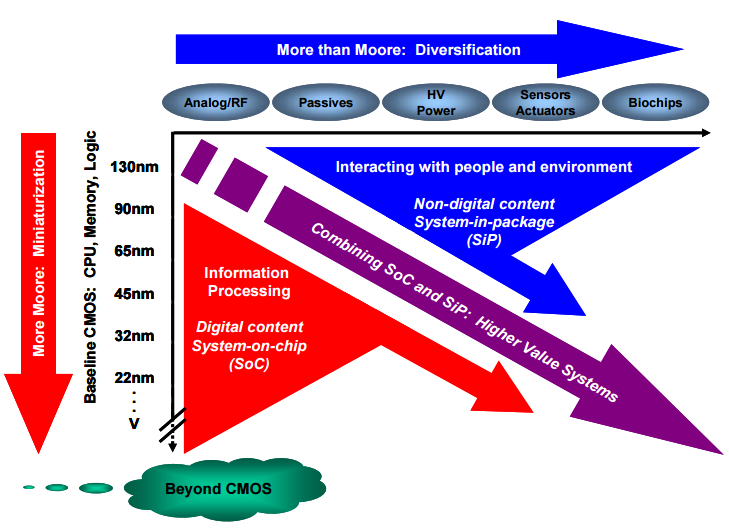
\includegraphics[width=\textwidth]{Figs/MoreThanMoore.png}
    \caption{\textit{More than Moore}. From ITRS~\cite{Arden2010}}
    \label{fig:moore}
\end{figure}

Meanwhile, those multiple components are evolving through time satisfying \textit{Moore's law} and getting miniaturised in a way that enables integrating various functionalities on the same chip, in which is called system-on-chip (SoC). Optimising both trends can achieve hatching new out-of-the-box solutions. Integrating such bulky diverse functionality devices can be achieved via exploring new ways of designing our computing units while being miniaturised. Such new directions employ on a bottom-up approach pointed by Feynman decades ago. Consequently, examining new trends in transistor material design, revolutionising the semiconductor field, becomes a necessity for enabling a combination of SiP and SoC for building higher value systems~\cite{Lemme2012}. As we have pointed above, candidate materials as graphene and other similar 2D promising materials can boost the electronic design within the more than Moore paradigm~\cite{Fiori2014nature, Fiori2015}.

After Novoselov's~\cite{Novoselov2004} effort on 2004, graphene research shed light upon potential applications due to its extraordinary properties. Specifically, a large pool of research has focused on integrating graphene in sensors~\cite{Lee2008, Geim2009, Smith2015, Smith2017}, supercapacitors~\cite{Liu2010, Yoo2011, Brownson2012}, biosensors~\cite{Shao2010, He2010}, radio frequency devices~\cite{Moon2009, Koswatta2011}, spintronics~\cite{Han2014} and photodetectors~\cite{Mueller2010, Lemme2011}. Such outstanding proven characteristics made graphene a hot topic for scientific research for the ultimate purpose of engagement within a diverse number of applications. 
%
%
\section{Research contribution}
In this work, we aim for the ultimate goal of examining graphene as a gas sensor theoretically; we elucidate the electronic structure studies of pristine single and double layered graphene residing on top of different substrates types as well as the adsorbates-graphene interactions and the influence coming from the substrate surface defects. We specifically investigate the interplay between the substrate common surface defects and the adsorbed water and carbon dioxide molecules on top of graphene sheets. We performed the studies via means of a first-principle \textit{ab-initio} method within dispersion corrected studies.
%
%
\section{Thesis organisation}
The thesis is compiled into seven chapters, detailed as the following:
\begin{itemize}
\item \textbf{Chapter 1} provides a background of the current trends in technology and motivation for this thesis work.
\item \textbf{Chapter 2} provides some insights on graphene theory.
\item \textbf{Chapter 3} focuses on the sensing mechanism of graphene and literature comparison with other materials in use.
\item \textbf{Chapter 4} presents some theoretical overview covering the method.
\item \textbf{Chapter 5} gives some insights on the used calculational parameters with an overview and recommendations of some technicalities related to the programs and method in use.
\item \textbf{Chapter 6} summarises the results of the related thesis's manuscripts.
\item \textbf{Chapter 7} outlooks the thesis work with some insights on some futuristic disciples and paths to go through.
\end{itemize}
\endinput

\chapter{Overview on Graphene}
\label{grapheneTheory}
A snippet of graphene's electronic, geometrical and mechanical properties is available in the following sections.
\section{Theoretical snippets on graphene}
A single layer of graphene consists of a monolayer of carbon atoms arranged in a 2D honeycomb-like structure. Within each layer, every carbon atom bonds to three neighbouring carbon atoms building a quasi 2D plan~\cite{Neto2009}, with sp$^\textrm{2}$ hybridisation between carbon atoms resulting in the single layer of graphene being intact~\cite{Neto2009}. Each carbon atom within the graphene sheet has a dangling bond as it is only connected to three nearby carbon atoms leaving a free valence electron forming a cloud of electrons covering the single graphene sheet, organised in half filled $\pi$ orbitals~\cite{Neto2009}. Such carbon atom's $\pi$ orbital interacts with its neighbours' counterparts forming conduction and valence bands~\cite{Bolotin2008, Morozov2008, Basu2012}. Thus, graphene's band structure is due to those $\pi$ orbital electrons with the conduction and valence bands intersecting at a point in the Brillouin zone named Dirac point. Fig. \ref{fig:G_BSTRUCT_structure} shows the Dirac point with zero bandgap, confirming the semimetal nature of graphene~\cite{Wallace1947} characterised by the Dirac electrons. As a result, these $\pi$ orbital electrons cause graphene to be sensitive to the surroundings, paving the road towards graphene-based sensors~\cite{He2012, Mzali2016} as detailed in section \ref{graphene:sensor} with further explanation in Chapter \ref{grapheneSensors}.

%
\begin{figure}
    \centering
    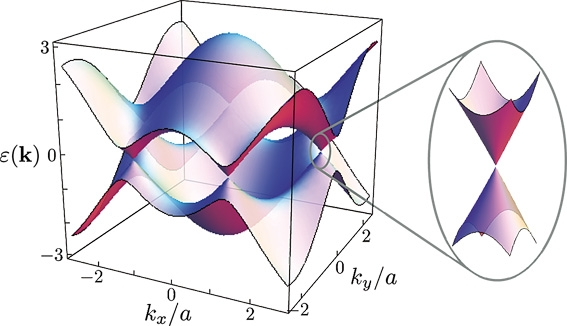
\includegraphics[width=\textwidth]{Figs/GrapheneBSTRUCT.png} %[scale=0.5,keepaspectratio]
    \caption{Graphene's band structure, from~\cite{dispersion}.}
    \label{fig:G_BSTRUCT_structure}
\end{figure}
%
Graphene monolayer sheet is considered one of the thinnest material ever known~\cite{Geim2007, Bunch2008}. Meanwhile, stacking graphene layers can take different stacking orders revealing different electronic properties. Two distinguished stacking orders can be either AA or AB stacking. AA stacking is semiconducting with a direct bandgap while AB stacking is a semi-metal with zero bandgap~\cite{Yakovkin2016}. In AA stacking order, the second layer's carbon atoms match precisely the top of the carbon atoms within the bottom layer. Within AB stacking, the carbon atoms within the top layer are on top of the centre of the honeycomb hexagon in the bottom layer. Figure (\ref{fig:G_BSTRUCT_structure_Stacking}) reveals the related band structure showing the band opening at the AA stacking order. Stability wise: AB stacking, which is the natural stacking order in graphite, is the more energetically favourable for graphene stacking orders~\cite{Yakovkin2016, Emroz2016, Cusati2017}. However, a forced opening of a bandgap in graphene's band structure can open many applications for graphene-based devices. Bandgap opening is possible through different techniques such as introducing strain in the graphene sheet~\cite{Zhen2008, Pereira2009, Cocco2010}, producing nanoribbons~\cite{Son2006, Han2007}, arrangement in different stacking orders~\cite{Ohta2006, Castro2007, Zhang2009}.
%
\begin{figure}
    \centering
    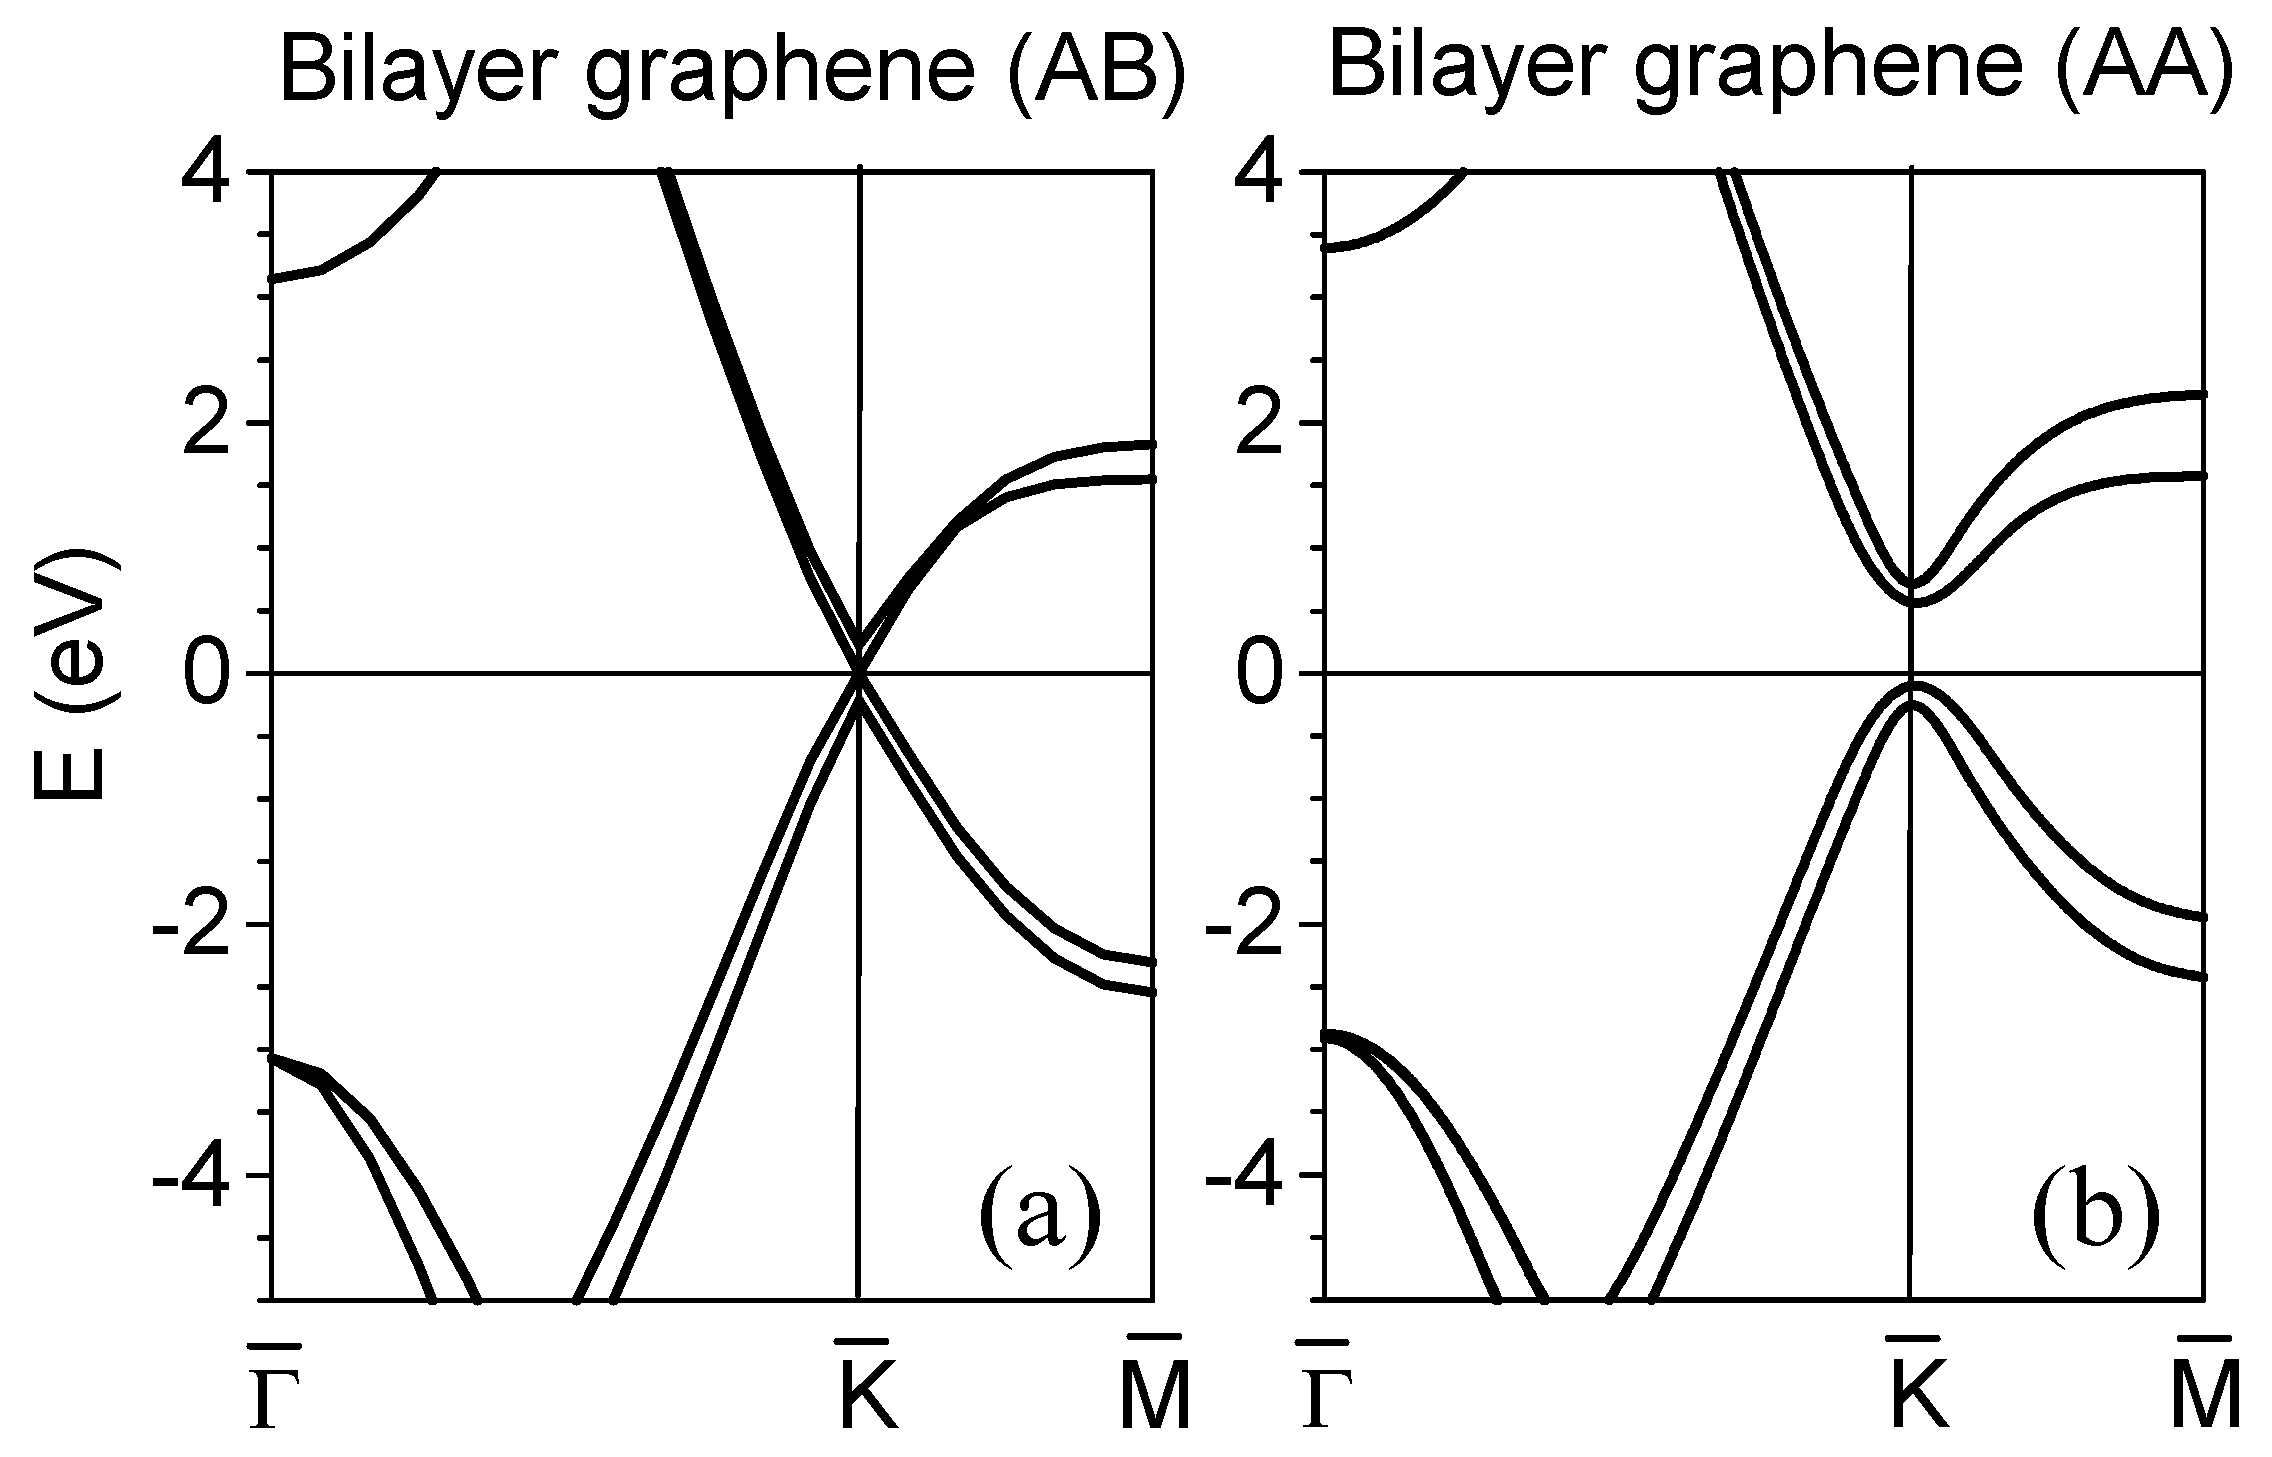
\includegraphics[width=\textwidth]{Figs/AA_AB_bandStructure.png}
    \caption{Band structure of AA and AB stacking orders in graphene bilayers. From~\cite{Yakovkin2016}}
    \label{fig:G_BSTRUCT_structure_Stacking}
\end{figure}

%
\subsection{Electronic properties}
\label{graphene:electronic}
Graphene shows ballistic transport due to the Dirac fermions that are massless quasiparticles~\cite{Geim2007}. Those massless quasiparticles are responsible for the resultant graphene's band structure (depicted in Fig. \ref{fig:G_BSTRUCT_structure}). They are a result of the graphene's electrons interacting with the hexagonal lattice periodic potential~\cite{Geim2007}. The Dirac equation~\cite{Gusynin2005, Novoselov2005, Zhang2005, Geim2007} does accurately model those particles. They are the graphene's charge carriers, and their relativistic properties are investigated experimentally via quantum Hall effect measurements~\cite{Novoselov2004, Novoselov2005}. Experimental studies~\cite{Novoselov2004, Hwang2007, Bolotin2008, Morozov2008, Vincent2010, Rahimi2014, Banszeruse2015} shows high mobility of 200,000 $\textrm{cm}^2 \textrm{V}^{-1}\textrm{s}^{-1}$. Moreover, graphene has been proven to have a low electronic noise, which in turn makes it an ideal material for detecting adsorbant gas molecules on its surface~\cite{Schedin2007}. Further details are discussed in the following chapter regarding the detection and sensing properties of graphene.
%
\subsection{Mechanical properties}
Graphene's mechanical properties are outstanding. Graphene has a Young modulus of 1 TPa~\cite{Lee2008, Lee2013} qualifying it to be part of nanoelectromechanical systems (NEMS) and electromechanical transducers~\cite{Smith2013, Smith2016a}. Applying strain of 20 \% is possible on graphene while maintaining the elastic region~\cite{Tomori2011}.  In turn, this opens the possibility for applications of graphene-based devices in the flexible electronics world~\cite{Fiori2014nature}. Moreover, applying strain can open a bandgap~\cite{Cocco2010}, with a shift in the Dirac point~\cite{Montambaux2009, Pereira2009, Li2014} and hence a bandgap in the resultant band structure of the graphene sheet. Furthermore, graphene well-reside on top of silica substrates~\cite{Koenig2011, Rudenko2011, Zhao2017} with strong adhesion forces dominated by van der Waals dispersive interactions. Finally, Graphene can build impermeable membranes, where it reported impermeability to standard gases~\cite{Bunch2008}. That is advantageous when designing graphene-based sensors.
%
\section{Graphene's applications}
Graphene faces some complications in the fabrication and design processes~\cite{Smith2016a, Fiori2014nature}, yet it is quite paying back concerning its wide applications integrity due to its extraordinary properties discussed earlier. This pool of applications for such a 2D material and other challenging 2D materials include, but not limited to, transistors~\cite{Lemme2012, Lemme2012a}, sensors~\cite{Smith2015, Smith2016a, Smith2017, Xuge2017, Feng2014, Wang2015, Yue2013, Zhao2014, Llobet2013}, transistor passivation~\cite{Smith2016}, energy harvesting~\cite{GRANDE2012}, faster charging batteries~\cite{Son2017}, potentiometer~\cite{Levesque2011}, supercapacitors and energy storage~\cite{Yoo2011, Brownson2012, Liu2010}, photodetectors~\cite{Mueller2010, Naiini2014, Lemme2011}, photodiodes~\cite{Riazimehr2017}, analog electronics~\cite{Fiori2014}, solar cells~\cite{Wang2008, Miao2012}, RF devices~\cite{Fiori2014nature}. Graphene's high optical transparency and high electronic conductivity open the door for touch screens~\cite{Ferrari2015} as a direct application of optoelectronic devices. Graphene applications can be extend towards NEMS systems~\cite{Chen2013}, such as graphene-based mechanical resonators~\cite{Bunch2007, Castellanos2015, Chen2013}, cantilevers~\cite{Conley2011}, pressure sensors~\cite{Smith2012, Smith2013b, Smith2014, Wagner2016}, magnetic field sensors~\cite{Dauber2015}, accelerometers~\cite{memsPatent}. All these applications fall into \textit{more than Moore} paradigm.
\subsection{Transistors}
Graphene can build the channel material in transistors for a promising post-silicon field effect transistor (FET) devices~\cite{Lemme2007, Smith2016a}. In such devices, the current flow in the central channel region from the source to the drain electrodes. This current is controlled by applying an external voltage to the gate electrode, which is shielded against the channel region by a dielectric. Applying means of external electric field can alter Graphene's resistance opening the possibilities for high-speed transistors~\cite{Schwierz2010}. Graphene can also be part of the base component of the transistor in graphene-based bipolar junction transistor (BJT)~\cite{Vaziri2013}. Graphene transistors can act as amplifiers as in~\cite{Han2011}. Graphene can be a promising building block for high-frequency devices for communication purposes~\cite{Smith2016a, Liao2012}. On a circuit design level, circuits designs can model and simulate graphene-based circuit components~\cite{Han2011, Wu2012, Thiele2010, Fregonese2013, Rodriguez2014}.
\subsection{Sensors}
\label{graphene:sensor}
Graphene has demonstrated potential in the sensor field due to its extraordinary properties, discussed in section \ref{graphene:electronic}. One of the main sensor applications here is the gas sensor in the form of solid-state devices featuring graphene~\cite{Moseley1997, Handbook_gas_sensing, Capone2003, Smith2016a, Elgammal2016Lic}. Such devices demonstrate competitive edge with sensing applications for more NEMS based applications. Chapter \ref{grapheneSensors} details the sensing action of graphene.
\section{Summary}
In summary, graphene has shown the potential to be a key player in advancing material science due to its remarkable properties being either electric or mechanical. Such properties allow graphene to be implemented in a wide range of device applications either being electronic or mechanical or consolidating both. Besides, being CMOS compatible allows it to be embedded in the current technologies seamlessly.
\endinput
\chapter{Graphene based sensors}
\label{grapheneSensors}

Here comes an overview of the sensory action of graphene with some insights on different factors behind the sensing mechanism. For a theoretical background for graphene and related properties, please refer to Chapter \ref{grapheneTheory}.
\section{Inauguration of graphene as a sensor}
Means of Atomic Force Microscopy experiments has ignited graphene's sensing behaviour visualising the first water adlayer on mica surface at ambient conditions~\cite{Xu2010} being a coating material on mica. Graphene's high selectivity to concentration changes for different ambient gases has enabled embedding it in sensory devices~\cite{Schedin2007, Yuan2013, Melios2017}. Graphene's sensitivity to gas molecules is mainly attributed to two factors: (1) graphene's $\pi$ orbitals~\cite{Neto2009} which interact with the adsorbates residing on top via van der Waals interactions, (2) graphene's high surface to volume ratio which is an advantage for all 2D materials. 

\section{2D materials as a gas sensor candidate}
By the millennium till now, vast number of materials have demonstrated gas sensing properties including low dimensional carbon-based materials as carbon nanotubes~\cite{Kong2000, Kuang2007}, graphene and its oxide~\cite{Ong2001, Schedin2007, Morozov2008,Fowler2009, Massera2011, Gautam2012, He2012, Dan2009, Ghosh2009, Ratinac2010, Sun2010, Yao2012, Basu2012, Liu2012, Gallouze2013, Nemade2013a, Borini2013, Yuan2013, Llobet2013, Saini2014, Zhang2013, Zhou2014, Hwang2014, Nakamura2015, Smith2015, Smith2016a, Smith2017, Xuge2017, Melios2017, Wu2015}. Recently, other 2D materials featuring a bandgap caught the attention as a promising candidate material for sensing devices. One example of such materials family is the transition metal di/tri-chalcogenides family (TMDCs/TMTCs)~\cite{Zhao2014}. For example, molybdenum disulfide has shown sensitivity to different gas molecules interacting on its monolayer~\cite{Yue2013, Zhao2014} showing sensitivity towards carbon monoxide/dioxide, ammonia, nitrogen monoxide/dioxide, methane, water molecules, nitrogen, oxygen and sulfur dioxide. Similarly, Dirac materials such as silicene have also demonstrated promising activity in the materials sensory behaviour~\cite{Feng2014}, showing sensitivity against a wide range of gases such as nitrogen monoxide/dioxide, sulfur dioxide, oxygen and ammonia, as well as formaldehyde~\cite{Wang2015}. Worth mentioning that Geim and Grigorieva' study on van der Waals heterostructures~\cite{Geim2013} has inaugurated the community to investigate further the resultant properties of stacking different 2D materials, revealing different properties which can have many applications, where sensors can be one of them~\cite{Mayor2016}. Interestingly, other low dimensional as metal oxides~\cite{Korotcenkov2007} or 1D materials as nanowires~\cite{Kong2000, Zhou2003, Wang2003} and tin oxide~\cite{Kuang2007} materials have proven sensing capabilities .
\section{Graphene as a gas sensor}

Graphene and other 2D materials have demonstrated sensing capabilities for an extensive collection of gases, both experimental and theoretical studies have focused on elucidating the different electronic properties within different ambient conditions emphasising different gases. The study in~\cite{Schedin2007} has experimentally enkindled the first graphene-based gas sensor achieving single molecule detection limit, in a way that the adsorbed gas molecules affect the charge carrier concentration and so the graphene device's resistance which is a direct measure of the device's sensitivity. Since then, studies focusing on various gases adsorption on graphene took place both theoretically and experimentally. Example of such gases are carbon dioxide and water molecules, where many of the studies examined their effect on graphene's electronic properties both theoretically~\cite{Ong2001, wehling2008doping, Wehling2008, Wehling2009, Ribeiro2008, Berashevich2009, Dai2009, Leenaerts2009, Yuan2010, Yang2011, Yoon2013, Freitas2011, Mishra2011, Voloshina2011, Deng2012, Paulla2013, Nemade2013a, Cazorla2013, Chen2014, Dutta2014, Xiao2014, Elgammal2017} and experimentally~\cite{Moser2008, Dan2009, Ghosh2009, Lu2009, Yavari2010, Yoon2011, Kalon2011, Yao2012, Yang2012, Tuan2013, Borini2013, Giusca2015, Tamilarasan2015, Smith2015, Hong2016, Smith2016a, Smith2016a, Melios2016, Panchal2016, Smith2017, Xuge2017, Melios2017}. 

Similarly, Graphene has showed sensitivity towards other gases such as carbon monoxide~\cite{Schedin2007, Ao2008, Zhang2009a}, oxygen~\cite{Yang2011, Yuan2013}, sulfur dioxide~\cite{Chen2014}, nitrogen monoxide/dioxide~\cite{Zhang2009dopants, Leenaerts2009, Dai2012, Panchal2016}, hydrogen sulfide~\cite{Yuan2010, Sharma2013} and ammonia~\cite{Zhang2009dopants, Leenaerts2009, Dai2009, Yuan2010}. Graphene sensing capabilities can be extended towards detecting complex bio-molecules~\cite{Lerner2017} such as DNA~\cite{He2010, Shao2010}, opening the capabilities for lab on chip applications for fast diagnosis or selectivity towards various bio-molecules~\cite{Barik2017}. This can enable graphene to enter the market of surface-based biosensors~\cite{Shao2010}. 
% %

Graphene's sensing behaviour towards adsorbates can differ according to graphene types~\cite{Smith2015}, thickness~\cite{Rafiee2012, Munz2015}, stacking orders~\cite{Melios2016}, defects~\cite{Banhart2011}, substrate effect~\cite{Hong2016, Wehling2008, Ashraf2016}. 
%
%
\section{Benchmarking against other materials based sensors}
Bench-marking graphene-based sensors against commercially available technologies are quite impressive. Honeywell\texttrademark developed a no expensive widely used humidity sensor based on polymer capacitive sensing mechanism~\cite{Delapierre1983}, with model code name (HIH-4000-001)~\cite{honeywell}. Its sensitivity can span the full relative humidity range yet achieves a response time of 10x and a recovery time of 40x making it pretty slower than graphene integrated CMOS resistive humidity sensor as demonstrated in~\cite{Smith2015}. The graphene-based humidity sensor does span 95\% relative humidity range, with a 5\% less than the commercial one.

Another example for well-developed humidity sensors in literature is the tin oxide~\cite{Kuang2007}, which is also resistive sensor and CMOS compatible. However, tin oxide based sensors do experience lower overall efficiency when compared to the graphene-based equivalent~\cite{Smith2015}, regarding the spanned relative humidity percentage range, response and recovery times and sensitivity to minute changes in humidity.
%
%
\section{Graphene's sensory action}
In the following subsections, we address different aspects that can play a role in graphene's sensing action towards different adsorbates.
%
%
\subsection{The nature of graphene-adsorbate interactions}
Environmental conditions and adsorbed molecules on top of graphene sheet do change the electronic properties of graphene regarding carrier concentration, resistance chance, work function and other properties~\cite{Kozbial2014, Panchal2016}. Pristine single-layered graphene is hydrophilic. However, it goes hydrophobic with stacked graphene layers~\cite{Munz2015} as per bernel stacked graphene (AB stacking). Moreover, the underlying substrate is proven to affect the hydrophilicity of the graphene sheet by doping mechanisms~\cite{Hong2016}. Adsorbates can dope the graphene sheet through p-doping~\cite{Panchal2016} as the adsorbates do attract electrons from graphene resulting in p-doping~\cite{Bollmann2015}. The sensing mechanism relies on changing the charge carrier concentration as well as charge carrier mobility~\cite{Melios2016, Melios2017tuning}.
%
%
\subsection{Effect of adsorbates on pristine graphene}
Adsorbates on top of pristine graphene have been investigated showing a charge transfer between the graphene sheet and the relaxed adsorbates on top. The charge transfer depends on the different orientations, geometries and relative positioning of the adsorbates~\cite{Leenaerts2008, Leenaerts2009}. For adsorbates of water type: the charge transport depends on the water molecule orientation, in which the charge transport is from the water molecule to the graphene sheet when the water's oxygen is the closest to the graphene sheet~\cite{Freitas2011} and reversed when the hydrogen atom is the closest~\cite{Leenaerts2008}. Adsorbates of water or ammonia existing on top of either single layered or bi-layered graphene sheets can, in some cases, open a bandgap opening in order of few tens of meV~\cite{Ribeiro2008}. The adsorbates orientations can depend on the graphene sheet charge where the hydroxylic bond within the water molecule does point towards the graphene sheet in case of negatively charged graphene~\cite{Tuan2013} and vice versa for positively charged graphene. Large concentrations of water adsorbates (forming icelike structures) on top of a pristine graphene sheet can result in comparably large net dipole moment accumulation, in which has a net doping effect on the graphene sheet leading to changing the electronic charges around the graphene sheet~\cite{Leenaerts2009}.

All in, the presence of water adsorbates concentration on both sides of the graphene sheet as well as its relative orientation either pointing towards the graphene sheet or opposite do have a resultant effective doping mechanism which changes the charge transfer to and from the graphene sheet~\cite{Leenaerts2009, Freitas2011, Tuan2013}. However, the change in the electronic structure is not dramatic when adsorbates are present~\cite{Wehling2008} and is quite minute as long as the study is concerned with the effect of adsorbates on pristine graphene. 
%
%
\subsection{Effect of adsorbates on defected graphene}
Defects can take place within the graphene sheet itself where common defects within the graphene sheet can be either categorised into point defects and 1D defects~\cite{Banhart2011}. Where point defects can involve Stone-Wales (SW) defect~\cite{Stone1986}, the typical single vacancy (SV)~\cite{Ugeda2010}, double and multiple vacancies, carbon adatoms, embedded foreign adatoms, substitutional impurities (introducing dopant atoms), defective topology and so on. While 1D defects can involve line defects, edge defects, and similar defects that result from separated domains within the graphene sheet characterised by different lattice orientations~\cite{Banhart2011}. Defects types can involve having unusual buckled or rippled graphene sites~\cite{Dutta2014}.

Graphene-based sensors featuring vacancy defects~\cite{Lee2016} has achieved sensitivity enhancement for various adsorbates signalling 33\% improvement for adsorbates of nitrogen dioxide and 614\% improvement for ammonia while compared to pristine graphene. Moreover, line defects can have a remarkable influence on graphene's electronic structure and hence the sensitivity towards adsorbates on top~\cite{Souza2018}. 

Experimental chemical and physical defects can alter the humidity sensitivity of graphene surfaces~\cite{SON2017defect} where the chemical defects (obtained by reactive ion etching) do have a more substantial effect on the sensitivity than the physical defects (via PMMA coating). 
%
%
\subsection{Effect of adsorbates on doped-graphene}
Graphene sheets sensing properties can depend on dopants existence within. Doping the graphene sheet itself changes the electronic and sensing properties~\cite{Zhang2009dopants, Panchal2016}, p-doping can be achieved via boron and nitrogen~\cite{Yuan2010, Deng2011, Deng2012}, gallium, germanium, arsenic and selenium dopants~\cite{Chen2014, Denis2014}, silicon doping~\cite{Zou2011}, aluminium doping~\cite{Dai2009, Sharma2013}. For example, aluminium-doped graphene has proven different electronic structure properties when adsorbing hydrogen fluoride molecules compared to pristine graphene~\cite{Sun2010}. Moreover, adsorption of hydrogen fluoride on top of Aluminium doped graphene has a chemisorption nature while it is physisorption for the pristine graphene case~\cite{Sun2010}. 

As doping graphene can alter the adsorption nature of adsorbates on top of a graphene sheet: an extensive study focusing on the adsorption nature of molecular hydrogen on top of graphene~\cite{Gallouze2013} has revealed that the adsorption can either be physisorption or chemisorption. Depends on graphene's dopant type: it is physisorption when the dopants are boron, iron, cobalt and nitrogen. While it is chemisorption when the dopants are hydrogen, beryllium, oxygen, sodium, aluminium, silicon, calcium, titanium, vanadium, chromium, nickel, copper and lithium.
%
%
%
%
\subsection{Effect of adsorbates on stacked graphene}
Different stacking orders in graphene do alter the carrier concentration and work function, while single-layered graphene is the most sensitive to different ambient conditions~\cite{Giusca2015, Panchal2016}. Adding only one layer resulting in bilayer graphene can decrease the sensitivity. Within bilayered-graphene, the bottom graphene layer is affected by charges coming from the substrate, while the top layer is affected by the adsorbates on top~\cite{Xuge2017}. The doping type, in this case, is also of acceptor type (p-doping)~\cite{Melios2016}.
%
%
%
%
\subsection{Effect of adsorbates on graphene with the influence of substrate}
Defects modifying graphene's electronic properties can extend towards the substrate surface defects in which the graphene sheet is residing on top~\cite{Wehling2008, Wehling2009, Elgammal2017}. Such commonly found substrate surface defects do contribute by inducing a net dipole moment with the presence of adsorbates on top of the graphene sheet. Such dipole moment accounts for a doping effect which results in changing the graphene's electronic structure and hence can alter the sensitivity~\cite{Wehling2008, Smith2015, Smith2017, Melios2017, Elgammal2017}. 

For example, adsorbates of oxygen with the presence of silica substrates dope the graphene sheet due to the couplings to the graphene sheet and the coupling between the graphene and the substrate~\cite{Ryu2010}. Oxygen molecules doping effect is of acceptor type (hole doping)~\cite{Liu2008}. Typically, such p-doping of graphene takes place when graphene exposes to regular atmospheric conditioning, i.e. exposure to water, carbon dioxide, oxygen and other ambient molecules in the air~\cite{Levesque2011, Anton2012}. Graphene p-doping action is not only due to the adsorbate in ambient conditions~\cite{Melios2017tuning} but also charges arising from the underlying silica substrate can induce such p-type doping of graphene~\cite{Melios2016}. Electronically, the underlying substrate surface defects can facilitate the doping effect by shifting the Dirac point by 0.5 eV as proven in~\cite{Levesque2011}. 

Moreover, altering the degree of hydrophobicity~\cite{Chen2014, Belyaeva2017} can directly affect the p-doping in graphene. For example, applying an electric field to the graphene-substrate system can alter the degree of hydrophobicity, resulting in a maximisation of the substrate induced doping~\cite{Hong2016}. The applied electric field shifts the Fermi level relative to the Dirac point changing the graphene doping from n-type to p-type doping.  
%
%
\section{Summary}
We have demonstrated a short overview of the influence of several parameters on graphene's sensing action with a big emphasis on the effects coming from the underlying substrate. As graphene has proven sensitivity to ambient conditions, we should give a careful treatment when constructing graphene-based sensory devices considering all the discussed parameters.

\chapter{Theoretical background}
\label{DFT-chapter}
In this chapter, an overview of the theory behind the calculations performed throughout the attached manuscripts is available. It introduces the Density Functional Theory (DFT) as well as snippets description on the used functionals and their development.
\section{The many-body problem}
The solution of any quantum mechanical problem is obtained by evaluating the eigenvalues and eigenfunctions of the Hamiltonian operator ($H\Psi=E\Psi$) formulated in equation \ref{manybodyH}. Since the exact solution of such equation for a many-body system is analytically impossible, therefore a series of approximations are to be applied. In this chapter, we briefly discuss basic theories and approximations, which formulates the density functional theory. The many-body Hamiltonian is formulated as in equation \ref{manybodyH}:
\begin{multline}
\hat{H}=\,\,\,\,-\,\,\,\,\overbrace{\frac{\hbar^2}{2}\sum_{I}{\frac{\nabla_I^2}{M_I}}}^\textrm{Nuclei K.E.}\,\,\,\,+\,\,\,\,\overbrace{{1 \over 2} \sum_{I \neq J}{\frac{Z_I Z_J e^2}{4\pi\epsilon_0\abs{\vec{R_I}-\vec{R_J}}}}}^\textrm{Nucleus-Nucleus Interaction}\,\,\,\,-\,\,\,\,\overbrace{\frac{\hbar^2}{2m}\sum_{i}{\nabla_i^2}}^\textrm{Electrons K.E.}\\ \,\,\,\,+\,\,\,\,\underbrace{{1 \over 2} \sum_{i \neq j}{\frac{e^2}{4\pi\epsilon_0\abs{\vec{r_i}-\vec{r_j}}}}}_\textrm{Electron-Electron Interaction}\,\,\,\,-\,\,\,\,\underbrace{ \sum_{i,  I}{\frac{Z_I {e^2}}{4\pi\epsilon_0\abs{\vec{r_i}-\vec{R_I}}}}}_\textrm{\, \, Electron-Nucleus Interaction}
\label{manybodyH}
\end{multline}

In the many-body Hamiltonian: the first term $\left[-\frac{\hbar^2}{2}\sum_{I}{\frac{\nabla_I^2}{M_I}} \right]$ represents the kinetic energy of all nuclei, each with mass $M_I$. The second term $\left[ {1 \over 2} \sum_{I \neq J}{\frac{Z_I Z_Je^2}{4\pi\epsilon_0\abs{\vec{R_I}-\vec{R_J}}}}\right]$ represents nucleus-nucleus interactions via Coulomb repulsive forces. The second term can be calculated efficiently using Ewald's summation method (which determines the electrostatic potential as well as the energy of point charges in a crystal~\cite{Prasanna2012}). The third term $\left[ -\frac{\hbar^2}{2m}\sum_{i}{\nabla_i^2} \right]$ represents the kinetic energy of electrons, each with mass $m$. The fourth term $\left[ {1 \over 2} \sum_{i \neq j}{\frac{e^2}{4\pi\epsilon_0\abs{\vec{r_i}-\vec{r_j}}}} \right]$ represents the Coulomb interaction within pairs of electrons (the so called Hartree interaction). The fifth and last term $\left[-\sum_{i,I}{\frac{Z_I e^2}{4\pi\epsilon_0\abs{\vec{r_i}-\vec{R_I}}}} \right]$ represents electron-nucleus Coulomb interactions. The $1/2$ in the electron-electron and nucleus-nucleus interactions is to correct for the double counting.
% when we do the sum over i not equal j
% we are counting 1 with 2 and 2 with 1
% so the same term we counted twice
% because it is the same interaction, so, we put 1/2

The first step to simplify the many-body Hamiltonian is to invoke the Born-Oppenheimer approximation, detailed in the following section.
\section{Born-Oppenheimer approximation}
\label{BO}
% Since the nucleus is at least two thousand times heavier than the electron, the motion of a nucleus is much slower than that of an electron. Therefore the first approximation to introduce here, is taking the kinetic energy of nuclei to be zero in equation~(\ref{manybodyH}). \\
The Born-Oppenheimer approximation~\cite{Born1998} (BO) simplifies the solution of the many-body Schr\"{o}dinger equation (equation~\ref{manybodyH}) as it separates the nuclear and electronic motion. This approximation leads to two wave equations. The first equation describes the electronic motion, which can be solved separately by further approximations to evaluate the electronic wave function and the ground state energy. The second equation provides a description of the motion of the nuclei.\footnote{The contents of this section and the upcoming sections closely follows the presentation in standard textbooks in the subject, e.g., ABC of DFT~\cite{ABCofDFT} and Density Functional Theory and the family of (L)APW-methods: a step-by-step introduction~\cite{planewaveBook}.} The final result is the simplified Born-Oppenheimer Hamiltonian described in equation~\ref{BOHamiltonian} below:
\begin{multline}
\hat{H}^{\text{BO}}=\,\,\,\,-\,\,\,\,\underbrace{\frac{\hbar^2}{2m}\sum_{i}{\nabla_i^2}}_\textrm{Electrons K.E.}\,\,\,\,+\,\,\,\,\underbrace{{1 \over 2} \sum_{i \neq j}{\frac{e^2}{4\pi\epsilon_0\abs{\vec{r_i}-\vec{r_j}}}}}_\textrm{Electron-Electron Interaction}\\
\,\,\,\,-\,\,\,\,\underbrace{\sum_{i,I}{\frac{Z_Ie^2}{4\pi\epsilon_0\abs{\vec{r_i}-\vec{R_I}}}}}_\textrm{Electron-Nucleus Interaction}\,\,\,\,+\,\,\,\,\underbrace{{1 \over 2} \sum_{I \neq J}{\frac{Z_I Z_Je^2}{4\pi\epsilon_0\abs{\vec{R_I}-\vec{R_J}}}}}_\textrm{Nucleus-Nucleus Interaction}
\label{BOHamiltonian}
\end{multline}

In atomic units, the Born-Oppenheimer Hamiltonian is expressed in equation~\ref{BOHamiltonianAtomic} with $\hbar=m_e=e=4\pi\epsilon_0=1$ as: 
\begin{multline}
\hat{H}^{\text{BO}}=\,\,\,\,-\,\,\,\,\underbrace{\frac{1}{2}\sum_{i}{\nabla_i^2}}_\textrm{Electrons K.E.}\,\,\,\,+\,\,\,\,\underbrace{{1 \over 2} \sum_{i \neq j}{\frac{1}{\abs{\vec{r_i}-\vec{r_j}}}}}_\textrm{Electron-Electron Interaction}\\
\,\,\,\,-\,\,\,\,\underbrace{\sum_{i,I}{\frac{Z_I}{\abs{\vec{r_i}-\vec{R_I}}}}}_\textrm{Electron-Nucleus Interaction}\,\,\,\,+\,\,\,\,\underbrace{{1 \over 2} \sum_{I \neq J}{\frac{Z_I Z_J}{\abs{\vec{R_I}-\vec{R_J}}}}}_\textrm{Nucleus-Nucleus Interaction}
\label{BOHamiltonianAtomic}
\end{multline}
\section{Hohenberg-Kohn theorems}
\label{HohenbergKohn}
The Born-Oppenheimer approximation simplifies the Hamiltonian of the many-body problem. Still, the number of degrees of freedom in the system is prohibitively large. The Hohenberg-Kohn theorems provide a further simplification through replacing all the complicated interaction by an external potential and formulating the ground state energy as a functional of the electronic density instead of dealing with the wavefunctions. This is the approach taken in the Hohenberg-Kohn (HK) theorems~\cite{Hohenberg1964}. Those theorems are considered the foundation of DFT. They are stated below as:

\textbf{Theorem I:} \textit{"For any system of interacting particles in an external potential} $V_{ext}(\textbf{r})$, \textit{the potential} $V_{\text{ext}}(\textbf{r})$ \textit{is determined uniquely, by the ground state particle density} $n_0(\textbf{r})$.\textit{"} \\
So equation \ref{BOHamiltonianAtomic} will be rewritten as:
\begin{equation}
\hat{H}=
-\frac{1}{2}\sum_{i}{\nabla_i^2} + {1 \over 2} \sum_{i \neq j}{\frac{1}{\abs{\vec{r_i}-\vec{r_j}}}} + \sum_{i}{V_{ext}(\vec{r_i})}
\label{extpot}
\end{equation}

\textbf{Theorem II:}
\textit{"The ground state energy could be expressed in terms of a universal functional of the electron density} $E[n(\vec{r})]$ \textit{valid for any external potential} $V_{\text{ext}}$. \textit{For any particular} $V_{\text{ext}}(\vec{r})$, \textit{the exact ground state state energy of the system is the global minimum value of this functional, and the density} $n(\textbf{r})$ \textit{that minimizes the functional is the exact ground state density} $n_0(\textbf{r})$.\textit{"} 

We can construct a universal function for the energy which contains a functional that does not depend on the external potential $V_{\text{ext}}(\textbf{r})$ and only depends on the density.
\section{The Kohn-Sham approach}
\label{KS}
The energy functional above contains a kinetic energy term. There is no known closed expression for this term at present, and thus the functional cannot be evaluated as it stands. With the Kohn-Sham approach, one can solve this problem. Achievable through the Kohn-Sham (KS) equations~\cite{Kohn1965} which replaces the difficult to solve the interacting many-body system with a solvable auxiliary non-interacting system. This formulation assumes that the ground state density of the original interacting system is equal to that of some chosen non-interacting system. The Kohn-Sham equation is formulated in the following equations.
\begin{eqnarray}
E[n]=F[n]+\int \!  \mathrm{d^3} {\textbf{r}}\, V_{ext}(\textbf{r})n(\textbf{r}) \\
\noalign {{Where}} 
F[n]=\underbrace{T_s[n]}_\textrm{K.E.} \, + \, \underbrace{ \, d^3\textbf{r}\,d^3\textbf{r}' \frac{n( \textbf{r} )\,n( \textbf{r}' )}{\abs{\textbf{r}-\textbf{r}'}}}_\textrm{Hartree} \, + \, \underbrace{ E_{xc}[n(\vec{r})]}_\textrm{Exchange-Correlation}
\end{eqnarray}

$F[n]$ is valid for any external potential $V_{\text{ext}}(\textbf{r})$. All terms here are solvable apart from the $E_{xc}[n(\textbf{r})]$ term.
\section{Exchange-correlation functionals}
\label{XC}
Next, we need to address the exchange-correlation term $E_{xc}[n(\vec{r})]$ in the energy functional. By solving the KS equations, the ground state energy and the density of the original interacting system are found with an accuracy limited by approximations utilised in the used exchange-correlation functional. In the process of modelling the exchange-correlation interactions, different approximations are applied each has its limitations. Such set of approximations are referred in the what so called Jacob's ladder~\cite{Perdew2001, Perdew2005}. The local density approximation (LDA) is one of the simplest approximations~\cite{Kohn1965, Barth1972}. $E_{xc}$ is substituted here with the homogeneous electron gas exchange and correlation energies as shown in equation~\ref{LDA}:
\begin{equation}
E_{xc}^{LDA}[n(\vec{r})] = \int \!   \, d\textbf{r} \, \epsilon_{xc}^{hom}[n(\vec{r})] \, n(\vec{r}) 
\label{LDA}
\end{equation}

Where $\epsilon_{xc}[n(\vec{r})]$ is the exchange-correlation energy density. 

A more accurate way to approximate the $E_{xc}$ is the generalized gradient approximation (GGA), where the functional includes not only the density but also the density gradient as illustrated in equation~\ref{GGAeqn}:
\begin{equation}
\label{GGAeqn} 
E_{xc}^{GGA}[n(\vec{r})] = \int \!   \, d\textbf{r} \, n(\vec{r}) \, f (n(\vec{r}), \nabla n(\vec{r}))
\end{equation}
Both exchange-correlation functionals; LDA and GGA has been lucrative in extracting structural, vibrational, elastic properties of materials governed by metallic, ionic, covalent bonds.

\section{Dispersion interactions}
Van der Waals (vdW) dispersion interactions and forces take place in various systems with organic, inorganic, polymeric or bio-organic nature~\cite{vdWreview}. vdW forces have a big influence in describing systems where surface molecules are weakly bounded to slabs~\cite{Rydberg2000, Langreth2005, vdWreview, Axel2014} or when addressing stacked layered materials~\cite{Geim2013}. In other words, it describes the physisorption of molecules on slab surfaces, in which is the case we deal mostly throughout this thesis' related manuscripts. Conventional DFT functionals do not count for such dispersive forces properly. 

\subsection{DTF-D empirical damped dispersion correction within the GGA}
As conventional functionals lack proper definitions for dispersive interactions, early attempts started by Wu and Yang~\cite{Wu2002} with the incorporation of an empirical dispersion correction term within some of the conventional functionals. After that Grimme~\cite{Grimme2004, Grimme2006} further developed the semi-empirical dispersive term. The corresponding vdW energy is added to the plain KS functional as a correction term, this term is assuming that the total dispersion interaction within solids or molecules is a summation of pairs by pairs contributions' from all atoms in the system. The energy is expressed in equation~\ref{Grimme} as:
%
\begin{eqnarray}
E_{\text{Grimme}} \, = \, E_{\text{KS-DFT}} \, + \, E_{\text{DFT-D}} \\
\noalign {{Where}}
E_{\text{DFT-D}} \, = \, - \, {s_6 \over 2} \, \sum_{i \neq j}{{C_6^{ij}} \over {R_{ij}^6}} \, f_{\text{damp}}(R_{ij}) \\
\noalign{Here $C_6^{ij}$ is the dispersion coefficient for each pair of atoms $i$ $\&$ $j$}
C_6^{ij} \, = \, \sqrt{C_6^{i}C_6^{j}} \\
\noalign{The empirical damping dispersion correction function $f_{\text{damp}}$ is given by:}
f_{\text{damp}}(R) = {1 \over {1+e^{-d(R/R_r-1)}}}
\label{Grimme}
\end{eqnarray}
%
As indicated in equation (\ref{Grimme}), each pair of atoms contributes in the summation by a term proportional to the inverse sixth power of their inter-atomic distance $R_{ij}$. The scaling factor $s_6$ differs according to the functional used, best parameterization is available with Becke's GGA~\cite{Becke1997}. The dispersion coefficient $C_6^{ij}$ as well as the damping function $f_{\text{damp}}(R)$ are preventing any diverge of the $E_{\text{DFT-D}}$ term at small $R_{ij}$ values. This approach has been referred to as Grimme correction or DFT-D where D here stands for dispersion. Wu and Yang's approach~\cite{Wu2002} developed the summation term without the scaling $s_6$ factor, that is why grimme approach is more advanced. 
\subsection{Non-local van der Waals functionals}
\label{nonlocalvdW}
The famous approximations to the exchange-correlation DFT functional previously discussed here are local and semi-local functionals, not allowing for a proper description of such non-local correlation contribution definition of forces and interactions. That was the case till Dion et al.~\cite{Dion2004} came up with a pure non-local functional describing such dispersive interactions as a stand-alone vdW DFT functional. The proposed formulism for the so called vdW functionals (vdW-DF) has an added vdW dispersion term. This overture led to definition of various version of vdW-DF functionals such as vdW-DF2~\cite{Lee2010DF2}, optB88, VV09~\cite{Vydrov2009}, VV10~\cite{Oleg2010}, rVV10~\cite{Sabatini2013}, the 'opt' functionals~\cite{vdWDFopt} (optPBE-vdW, optB88-vdW, and optB86b-vdW).
\subsection{vdW functional formulation}
Upon inauguration of the original "vdW-DF" functional by Dion et al.~\cite{Dion2004} in 2004 including vdW interactions, Thonhauser et al.~\cite{thonhauser2007van} implemented the method later on 2007 self-consistently. The exchange-correlation term is defined as stated in equation (\ref{vdWeqn1}) where the exchange term is defined within the GGA exchange energy $E_{\text{x}}^{\text{GGA}}[n(\vec{r})]$ obtained from the revPBE functional definition~\cite{Zhang1998}. Such exchange term doesn't have any spurious binding. Meanwhile, the local correlation energy $E_{\text{c}}^{\text{LDA}}[n(\vec{r})]$ is obtained within the LDA definition for the correlation. LDA exchange was avoided due to its additional attraction contribution which can falsify the results. Finally, the non-local explicit correlation energy $E_{c}^{\text{nl}}$ term is added involving all the necessary machinery for vdW forces. 
\begin{equation}
E_{\text{xc}}[n(\vec{r})] \, = \, E_{\text{x}}^{\text{GGA}}[n(\vec{r})] \, + \, E_{\text{c}}^{\text{LDA}}[n(\vec{r})] \, + \, E_{c}^{\text{nl}}[n(\vec{r})]
\label{vdWeqn1}
\end{equation}
The simplest form for the non-local correlation energy part to the vdW-DF functional is defined in equation (\ref{vdWeqn2}).
\begin{equation}
E_{c}^{\text{nl}}[n(\vec{r})] \, = \, {\hbar \over 2} \, \int \!   \, d\vec{r} \, \int \!   \, d\vec{r}' \, n(\vec{r}) \, \Phi(\vec{r},\vec{r}') \, n(\vec{r}') 
\label{vdWeqn2}
\end{equation}
where the kernel $\Phi(\vec{r},\vec{r}')$ is a general function depending on $\vec{r}-\vec{r}'$ as well as the densities $n(\vec{r})$, $n(\vec{r}')$. 

With the introduction of vdW-DF by Dion et al.~\cite{Dion2004}, dispersion interactions are taken into consideration within the \textit{ab-initio} approach with no empirically introduced parameters as done in grimme correction~\cite{Grimme2006}. The other vdW functionals that followed Dion's definition are significantly improving the accuracy of the method. One of the main concerns in Dion's approach was the over-binding issue due to the role of the exchange term defined in revPBE functional. This revPBE's exchange term is providing the exchange term in the vdW functional definition formulated in equation (\ref{vdWeqn1}).
\subsection{van der Waals functional development}
Here comes an overview of such range of functionals, introduced for the ultimate purpose of improving the accuracy of Dion et al.'s~\cite{Dion2004} vdW-DF original functional according to the following:
\subsubsection{vdW-DF$^{\textrm C09_x}$}
Cooper et al.~\cite{Cooper2010} have introduced the vdW-DF$^{\textrm C09_x}$ with a focus on improving the exchange part by minimising the short-range exchange repulsion due to revPBE acting quite repulsive in such vdW regime~\cite{Gulans2009, Murray2009}. Such changes led to a better agreement with results reported in the S22  benchmarking database~\cite{Jurecka2006} (considered as a "gold standard" database): the benchmarking revealed a 9\% deviation compared to 17\% scored by the original vdW-DF with the revPBE exchange term.
\subsubsection{vdW-DF2}    
Furthermore; Lee et al.~\cite{Lee2010DF2} brought a second version of the Dion's vdWDF calling it vdW-DF2 where they focused on improving both the exchange and the non-local terms in the exchange-correlation definition in equation (\ref{vdWeqn1}). They used Murray's et al.~\cite{Murray2009} updated exchange version of Perdew's~\cite{Perdew1986}. Murray's exchange included the revised version of the PW86 functional (revPW86). They also further tuned the kernel $\Phi(\vec{r},\vec{r}')$ contributing in the non-local term. Lee et al. made a comparison with experimental results as well as the S22 benchmarking database in~\cite{Jurecka2006} and got quite good agreement and better accuracy compared to the original vdW-DF.
\subsubsection{opt- vdWs}
As the effort continues towards improving the original vdWDF; Klimeš et al.~\cite{vdWDFopt} introduced the new 'opt-' family of vdW functionals named optPBE-vdW and optB88-vdW where they examined a pool of exchange functionals to replace the revPBE exchange term in equation \ref{vdWeqn1}. Klimeš's et al. had achieved a satisfactory target, regarding satisfying energy accuracy, of 43 meV or 1kcal/mol, which is considered as a "chemical" accuracy. The proposed functional has, in turn, a significant accuracy improvement compared to the corresponding original vdW-DF, signalling accuracy of 60 meV, while compared to the S22 benchmarking database~\cite{Jurecka2006}.
\subsubsection{VV10}
Furthermore, a continual effort was made in improving the accuracy by fine-tuning the non-local correlation energy, introducing the vdW-DF-04 and vdW-DF-09 functional by Vydrov and van Voorhis~\cite{Oleg2009improving, Vydrov2009, Vydrov2010dispersion}. Their effort was concluded with the introduction of the VV10~\cite{Oleg2010}. In which, they introduced an adjustable parameter in the non-local correlation kernel $\Phi(\vec{r},\vec{r}')$ definition making it quite more efficient when comparing to their previous efforts, regarding both computational cost as well as the resultant accuracy. Worth mentioning, they carried out a benchmarking study~\cite{Vydrov2012benchmarking} comparing two versions of their VV10 functional (VV10 and LC-VV10) as well as with the famous vdW-DF2 revealing better accuracy with a comparable CPU time.
\subsubsection{vdW-DF-cx}
Moreover, Berland et al.~\cite{Berland2014vdWxc} had introduced the vdW-DF-cx functional with a so-called LV-PW86r exchange functional which in turn relies on the Perdew-Wang-86~\cite{Perdew1986, Murray2009} exchange energy. The term -cx- here stands for consistent exchange while the term -LV- stands for the Langreth-Vosko gradient expansion. They are parameterised in the functional definition. They had benchmarked the functional with experimental and RPA results~\cite{Bjorkman2012PRL, Bjorkman2012areWeReady} for various bulk structures, graphite and the layered dichalcogenides. We have chosen this functional in some of the publications presented in this thesis due to the agreement with experimental and RPA reported values for graphite calculations as shown in Berland's work~\cite{Berland2014vdWxc} motivating for the functional. Moreover, Lebègue et al.~\cite{Lebegue2010PRL} bench-marked their RPA results with both the quantum Monte Carlo and a range of experimental values. It is worth to note that experimental results reported for graphite systems can span a wide range of values depending on different parameters and conditioning concerning experiments; thus a comparison with quantum Monte Carlo calculations can provide a proper benchmark for graphite~\cite{Spanu2009PRL}.
\subsubsection{spin polarized vdW}
Thonhauser et al.~\cite{Thonhauser2015PRL} had introduced non-local magnetic interactions in which can be applied on spin-polarised systems. They developed the spin-polarised version of vdW-DF1, vdW-DF2 and vdW-DF-cx prefixing them with -s- standing for spin-polarised as svdW-DF1, svdW-DF2, svdW-DF-cx. It is also in agreement with the other functionals in a systematic approach presented in~\cite{Lee2015systematic}. They had justified their implementation against experimental and quantum Monte Carlo. They have also implemented their method in Quantum Espresso~\cite{Giannozzi2009} package as well and studied an example of graphene deposition on nickel 111 surface cut revealing exact match with the experimental value using the svdW-DF-cx (depicted in Fig. \ref{fig:svdW}a) making it suitable for such slab based systems. Thonhausers's results are in agreement with earlier results from Hamada and Otani~\cite{Hamada2010} showing a confirmation but with the proposed functional by Cooper's~\cite{Cooper2010} emphasising the exchange term (depicted in Fig. \ref{fig:svdW}b). Berland et al. in a later study~\cite{vdWreview} benchmarked the vdW-DF-cx functional with peer functionals as well as with quantum Monte Carlo results from~\cite{Spanu2009PRL} and experimental value revealing strong agreement with both benchmarks as depicted in figure \ref{fig:svdWGraphite}.
\begin{figure}
    \centering
    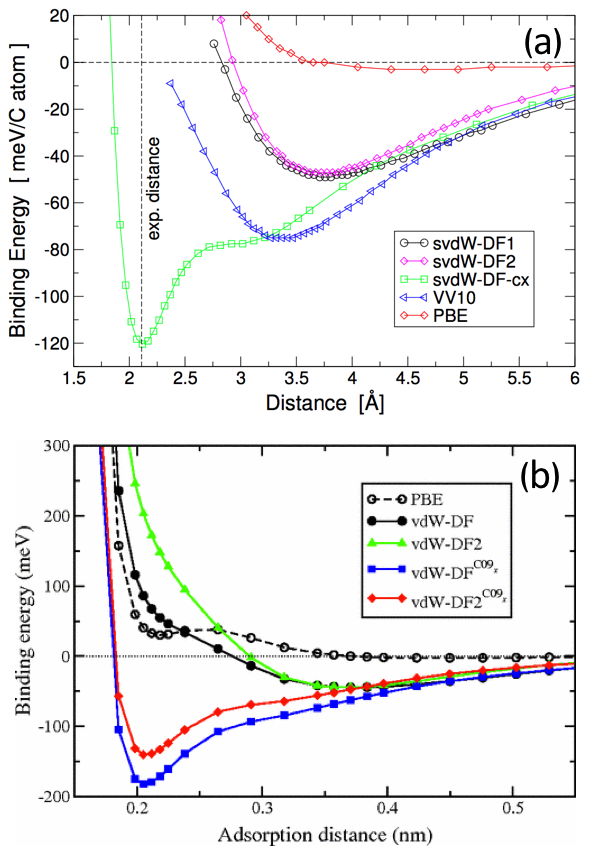
\includegraphics[scale=1.0,keepaspectratio]{Figs/svdW.png}
    \caption{(a) Taken from supplementary material given by~\cite{Thonhauser2015PRL} depicting the equilibrium distances and binding energies for graphene on the Ni 111 surface. Examined with different spin polarised vdW functionals and comparing it with other non-local functionals. The experimental value for equilibrium binding distance is taken from~\cite{Gamo1997}. (b) Taken from~\cite{Hamada2010} showing the same curve as in (a) but emphasising Cooper's version of functional~\cite{Cooper2010}, these calculations are spin-polarised as well}
    \label{fig:svdW}
\end{figure}
\begin{figure}
    \centering
    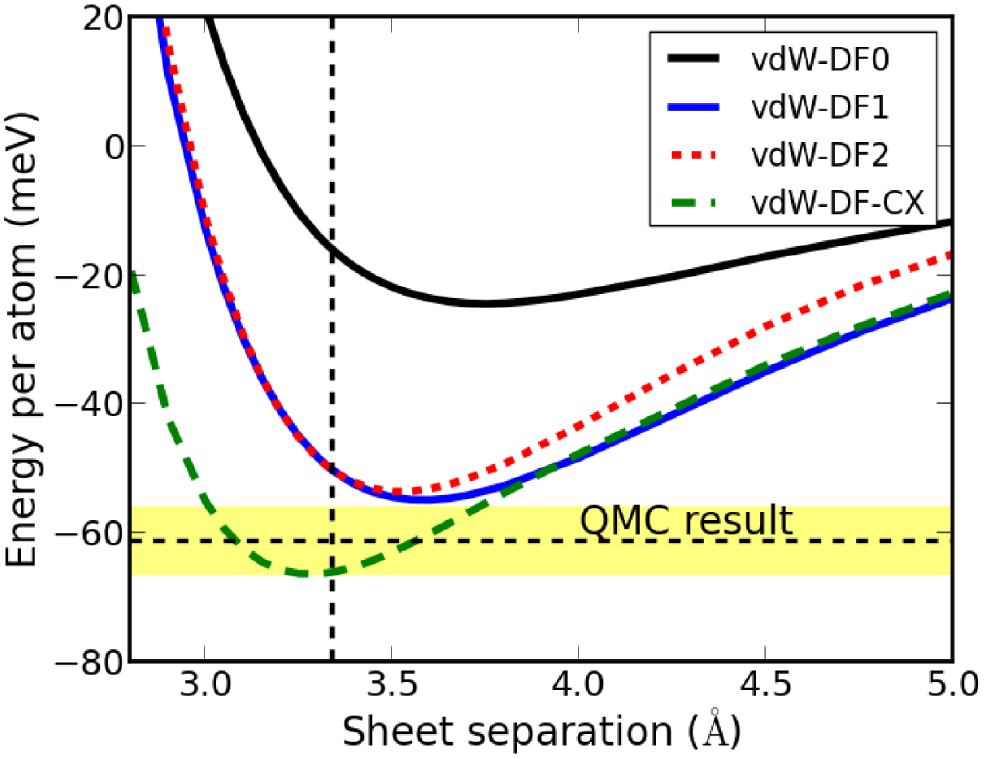
\includegraphics[scale=1.0,keepaspectratio]{Figs/svdWGraphite.jpg}
    \caption{Taken from~\cite{vdWreview} benchmarking the performance of the vdW-DF-cx functional versus the earlier versions of vdW-DFs, the experimental value represented in the vertical dashed line and the quantum Monte Carlo and RPA result (from~\cite{Lebegue2010PRL, Spanu2009PRL}) with the horizontal dashed line with yellow error bar regions. The figure is a result of a calculation of the inter-layer separation values within graphite.}
    \label{fig:svdWGraphite}
\end{figure}

As the non-local correlation term contains a double spatial integral as shown in equation (\ref{vdWeqn2}) resulting in six-dimensional integrals, it gets quite computationally expensive calculating it the way it was introduced either none-self-consistently~\cite{Dion2004} or self-consistently~\cite{thonhauser2007van} making it an $\mathcal{O}(n^2)$ problem. Román-Pérez together with José M. Soler\cite{NlogNalgorithm} calculated the integral self-consistently by factorising the integration kernel and use the fast Fourier transforms to evaluate the self-consistent potential, total energy, and atomic forces resulting in a reduced computational complexity of $\mathcal{O}(n\log{}n)$ operations. Regarding calculational time, this method is $\approx 10^3$ times less expensive than the original implementation and $\approx 10$ times costly when compared to the PBE cost. This algorithm is widely implemented in the different DFT codes nowadays. Sabatini et al.~\cite{Sabatini2013} had also introduced algorithm efficiently implementing the VV10 functionals, introducing the rVV10 functional.

As a quick overview on the efficiency of the proposed non-local functionals and benchmarking their results with experimental results: Björkman et al.~\cite{Bjorkman2012areWeReady} calculated the energy per unit area of the surface of the hexagonal hafnium ditelluride (HfTe$_{\textrm 2}$) TMDC for a wide range of different c lattice constant values. They got minima at the experimental value via the VV10 functional~\cite{Oleg2010} as well as a close performance achieved by the DFT-D correction~\cite{Grimme2006} as depicted in Fig. \ref{fig:vdWcomparison}a. HfTe$_{\textrm 2}$ is a layered semi-metal as graphene where its layers are intact together via vdW interactions. Similarly, Berland et al.~\cite{Berland2014vdWxc} benchmarked the vdW-DF-cx with the experimental as well as the accurate RPA results for graphite lattice constants revealing excellent agreement as shown in Fig. \ref{fig:vdWcomparison}b. 
\begin{figure}
    \centering
    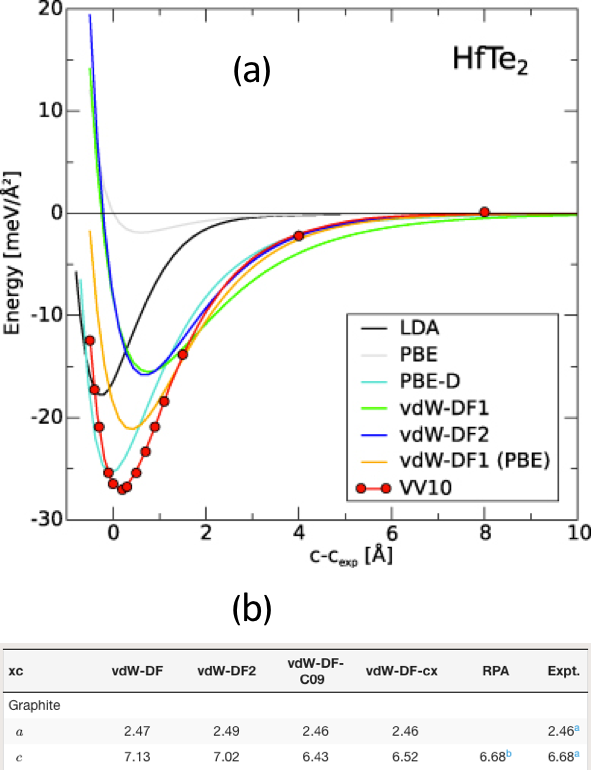
\includegraphics[scale=1.0,keepaspectratio]{Figs/vdWcomparison.png}
    \caption{(a) excerpt from~\cite{Bjorkman2012areWeReady} showing the performance of various dispersion functionals dealing with the dispersion forces governed by vdW showing both the densities overlaop pauli repulsion compression side as well the vdW attraction slope. (b) taken from~\cite{Berland2014vdWxc} showing results from differnet vdW functionals on graphite lattice constants.}
    \label{fig:vdWcomparison}
\end{figure}
In conclusion, The vdW functionals have been proven to be a not very expensive regarding computational time except for some complicated accurate versions, complicating the kernel. They give a promising solution for high accuracy calculations achieving the so-called "chemical" accuracy. That, in turn, can help \textit{ab-initio} scientists who are always concerned about solving the optimisation problem of accuracy versus calculation cost. Of course, with further development in computing technologies, scientists can shift their interest towards the exact method of quantum Monte Carlo (QMC) or random phase approximation (RPA). The open question is whether it is crucial to the specific problem under study or not. Worth mentioning, comparing DFT results with QMC or RPA is advantageous where we can avoid experimental uncertainties and contributions from the thermal motion that are not dealt in BO approximation.
\subsection{vdW and 2D materials}
As discussed in previous paragraphs, vdW functionals had a long run of success if we benchmark it with accurate methods in quantum Monte Carlo and PRA. In 2D materials, the uses of vdW functionals are materialised in describing the physisorption of molecules towards 2D surfaces, including graphene, TMDC and other valleytronics materials. That has been studied extensively in literature~\cite{Berland2013, Moses2009, Kleis2008, Berland2011,Joel2012, Bergvall2011, Svetla2010, Duy2012, Lee2011H2Cu111, Elias2012, Jiang2009, COOPER201234, Bjork2010, Martin2011}.
\section{Planewaves and pseudopotentials}
\label{planewaves}
In the thesis' related manuscripts, we used planewaves together with pseudopotentials, where planewaves is a type of basis set. With the help of a basis set, an arbitrary function (for example a charge density of a wave function) can be written as a sum of the basis functions weighted with coefficients. 

Equation~\ref{PWeigenfunc} expands the eigenstates in terms of an infinite number of plane waves with corresponding coefficients. $c_{\vec{K}}^{n,\vec{k}}$.
\begin{equation}
\psi_{\vec{k}}^{n}(\vec{r}) \, = \, \sum_{\vec{K}}c_{\vec{K}}^{n,\vec{k}}e^{(\vec{k}+\vec{K}).\vec{r}}
\label{PWeigenfunc}
\end{equation}

It is impossible to numerically evaluate an infinite number of coefficients for the basis set. Therefore the solution is limited to $\vec{K}$ by specifying a limiting value $\vec{K}_{\text{max}}$, which is the radius of a sphere in the reciprocal space whose centre is the origin. Thus, the limiting factor for all the $\vec{K}$ is set to $\vec{K} \leq \vec{K}_{\text{max}}$. The corresponding free electron energy is called the \textit{cut-off energy} which is expressed in equation~\ref{cutoffE} as:
\begin{equation}
E_{\text{cut-off}} \, = \, {{\hbar^2 K_{\text{max}}^2}\over{2m_e}}
\label{cutoffE}
\end{equation}
Here, $m_e$ is the electron mass.
\subsection{Pseudopotentials and vdW functionals}
As the electronic wave functions are very steep in the close neighbourhood of the nucleus and the limitation introduced by choosing a plane wave cutoff will cause high inaccuracy. Replacing the potential in the close vicinity of the nucleus with a pseudopotential that models the electronic wave functions properly in the interstitial region can be a good solution to the inaccuracy issue. Since most of the chemical bonding appears away from the nucleus in the inter-atomic region, the result of using pseudopotentials has a much lower computational cost for the same accuracy.

Ikutaro et al.~\cite{Ikutaro2011} have done a fascinating study comparing vdW electronic structure calculations performed using pseudopotentials generated with PBE functional versus pseudopotentials generated with consistent vdW functionals, they found out that the binding distances are slightly underestimated with pseudopotentials generated with PBE functional, while the binding energies are slightly overestimated. Meanwhile, the electronic structure regarding band structures is not altered. These differences are still in the range of the chemical accuracy with an error of 36 meV. Thus, it is safe and considerably still accurate to use pseudopotentials generated by PBE within vdW electronic structure calculation. It is a common practice to use PBE pseudopotentials as the vdW-DF non-local functionals utilise their exchange term.
\section{Summary}
In summary, we have enlightened the basis of DFT and how dispersion interactions are treated within. Dispersion interactions are essential to be considered when dealing with layered materials and describing adsorption properties. As there are several ways to describe it, thus, we choose the one suitable for the specific system under study.
\endinput
\chapter{Method and calculational details}
\label{chapter:calcDetails}
Here comes an overview of the used DFT code, pseudopotentials, cutoffs and other details related to the calculations setup.
\section{Used code}
All the numerical simulations throughout this thesis' manuscripts have been performed using density functional theory (DFT)~\cite{Hohenberg1964, Kohn1965}. The Kohn-Sham equation described in section \ref{KS} has been solved within the formalism of the planewave basis sets and pseudopotentials~\cite{Vanderbilt1990}. We have carried out the calculations using the integrated open-source software distribution suite of Quantum ESPRESSO~\cite{Giannozzi2009} abbreviated (QE) which is an integrated suite of electronic structure calculations codes based on DFT using planewave basis sets and pseudopotentials. It can be downloaded from~\cite{QE_link} for free.
\section{Used pseudopotentials}
Pseudopotential choices vary throughout this thesis' manuscripts. Here comes a brief overview of the chosen ones: 
\begin{itemize}
    \item \textbf{The HSCV pseudopotentials library}~\cite{PP_HSCV}: It is norm-conserving pseudo-potentials. It stands for Hamann, Schluter, Chiang and Vanderbilt (HSCV). We have used it at a tested cutoff of 130 Ry. We used it in the manuscripts representing Papers \hyperref[P1]{$\Rmnum{1}$}, \hyperref[P4]{$\Rmnum{4}$}, \hyperref[P5]{$\Rmnum{5}$} with a planewave energy cutoff value of 130 Ry.
\item \textbf{The GBRV pseudopotentials library}~\cite{Garrity2014}: it is ultrasoft pseudopotentials downloadable from Rutgers database~\cite{GBRVdatabase}. It is highly accurate and computationally inexpensive open-source pseudopotential library designed and optimised for use in high-throughput DFT calculations. It has relatively low recommended cutoffs of 40 Ry for the planewave and 200 Ry for the charge density. It has been used in the manuscripts representing Papers \hyperref[P2]{$\Rmnum{2}$}, \hyperref[P7]{$\Rmnum{7}$} with the recommended cutoffs.
\item \textbf{The SSSP pseudopotentials library}\cite{SSSP}: It is an ambitious pseudopotentials curation effort done on most of the commonly available pseudopotential libraries for the QE suite leading to the identification of optimal pseudopotentials. In which, they are classified into either efficient (relatively faster) or accurate choices of pseudopotential sub-libraries. Energy cutoff values, theorised in section \ref{planewaves}, are provided for almost every element in the periodic tables, where both cutoffs for the wavefunction and charge-density were chosen according to convergence tests concerning cohesive energies, stresses and phonon frequencies performed for each element~\cite{SSSP}. The SSSP library was originally constructed within the framework of AiiDA~\cite{Pizzi2016, AiiDA_link}, an open-source platform to manage and automate scientific computational work-flows without human intervention. The SSSP pseudopotentials were exhaustively tested and chosen from various sources~\cite{Garrity2014, Kucukbenli2014, Dalcorso2014, Schlipf2015, Willand2013, Topsakal2014}. The accuracy sub-library has been bench-marked providing -to date- the best overall agreement with the all-electron codes results~\cite{Lejaeghere2014, Lejaeghere2016}. This SSSP accuracy library has been used in the manuscript representing Paper \hyperref[P3]{$\Rmnum{3}$} with the assigned recommended cutoffs.
\item \textbf{ONCV pseudopotentials library}~\cite{Schlipf2015}: It is norm-conserving scalar relativistic pseudopotentials, it stands for Optimized Norm-Conserving Vanderbilt. It is considered as the updated version of the HSCV with an efficient lower cutoff, 60 Ry, about half the value needed for HSCV regarding the same systems. This pseudopotential was the choice in the manuscript representing Paper \hyperref[P6]{$\Rmnum{6}$}, where it has been used at the recommended cutoff of 60 Ry.
\end{itemize}
\section{Used functionals}
As we have pointed before in the subsection \ref{nonlocalvdW} for the importance of modelling vdW interactions, we used either non-local vdW functionals~\cite{Berland2014vdWxc} or semi-empirical corrections~\cite{Grimme2004, Grimme2006} to account for the dispersive interactions taking place within the slabs, graphene sheets and the available adsorbates on top.
\section{Systems modelling}
All systems under study within all the manuscripts involved slabs with incorporated vacuum to avoid any interaction within periodic images constructed by the code. In the manuscripts systems, we treated both slab surfaces symmetrically where the termination end of the top and bottom of the slab are identical. That serves the purpose of cancelling any resultant intrinsic dipole moment resulting from the slabs in case they are treated asymmetrically. We built the slabs to be quite thick resulting in bulk-like middle layers inside the slabs. We followed another approach in the manuscript representing Paper \hyperref[P3]{$\Rmnum{3}$}, which is the dipole correction~\cite{Bengtsson1999} method implemented in the QE package. Such correction can compensate for the artificially produced field within the supercell's vacuum by imposing a saw-like potential cancelling the artificially generated one taking place in the vacuum.
\section{Other calculational details}
\begin{itemize}
    \item Within most of the manuscripts in this thesis, we have generated QE input files from bulk Crystallographic Information File (CIF) files via the CiF2CeLL utility code~\cite{Torbjorn2011, CIF2CELLlink}. We fetched most of those CIFs from the materials project database~\cite{Anubhav2013, MaterialsProjectLink}. Those CIFs are available after undergoing satisfactory relaxations processes through their automated machinery available at the Materials Project repositories. Materials project uses the ICSD library~\cite{Bergerhoff1983, ICSDLink} as a source of the structures being fed into their computational workflows.
    \item We calculated the charge transfer using the Bader charge analysis~\cite{Bader1994} via a utility code computationally implemented in~\cite{Henkelman2006, Tang2009}. 
    \item We computed Löwdin charge analysis~\cite{Lowdin1955} as implemented in QE package.
    \item We used the visualisation tools xCrysden~\cite{Kokalj1999} and VESTA~\cite{Momma2011} for visualising system components and charge density differences. Both utilities can be downloadable from~\cite{xCrysdenLink} and~\cite{VESTALink}
\end{itemize}
\endinput
\chapter{Results and discussion}
\label{Results-discussion-chapter}
In this work, we discuss potential \textit{more than Moore} applications of graphene-based devices through theoretical studies associated with experiments for real insights on the functionality of the sensory action of graphene. We emphasised the significance of humidity and carbon dioxide on graphene-based devices from a first-principle calculations point of view as well as the effect coming from the substrate. We also highlighted the possibility of passivating such sensors and making the device non-functional for serving the purpose of better integrity into \textit{more than Moore} applications.  

The results are presented in full in the attached seven manuscripts as in five published articles and two in the manuscript format under submission. Here, we provide a summary of these papers and how they connect.

To study graphene-based sensors theoretically, we carried out DFT calculations for examining and simulating the effect of the presence of adsorbates of carbon dioxide and water molecules on top of graphene. We constructed the supercells and set up the calculations in light of the calculational details discussed in Chapter \ref{chapter:calcDetails}. We calculated the binding distances, energies, charge transfer, charge density differences (CDD) and density of states for supercells of pristine graphene with adsorbates on top while the substrate is intact. We took care of the dispersive forces as reviewed in Chapter \ref{DFT-chapter}. 

\begin{figure}
    \centering
    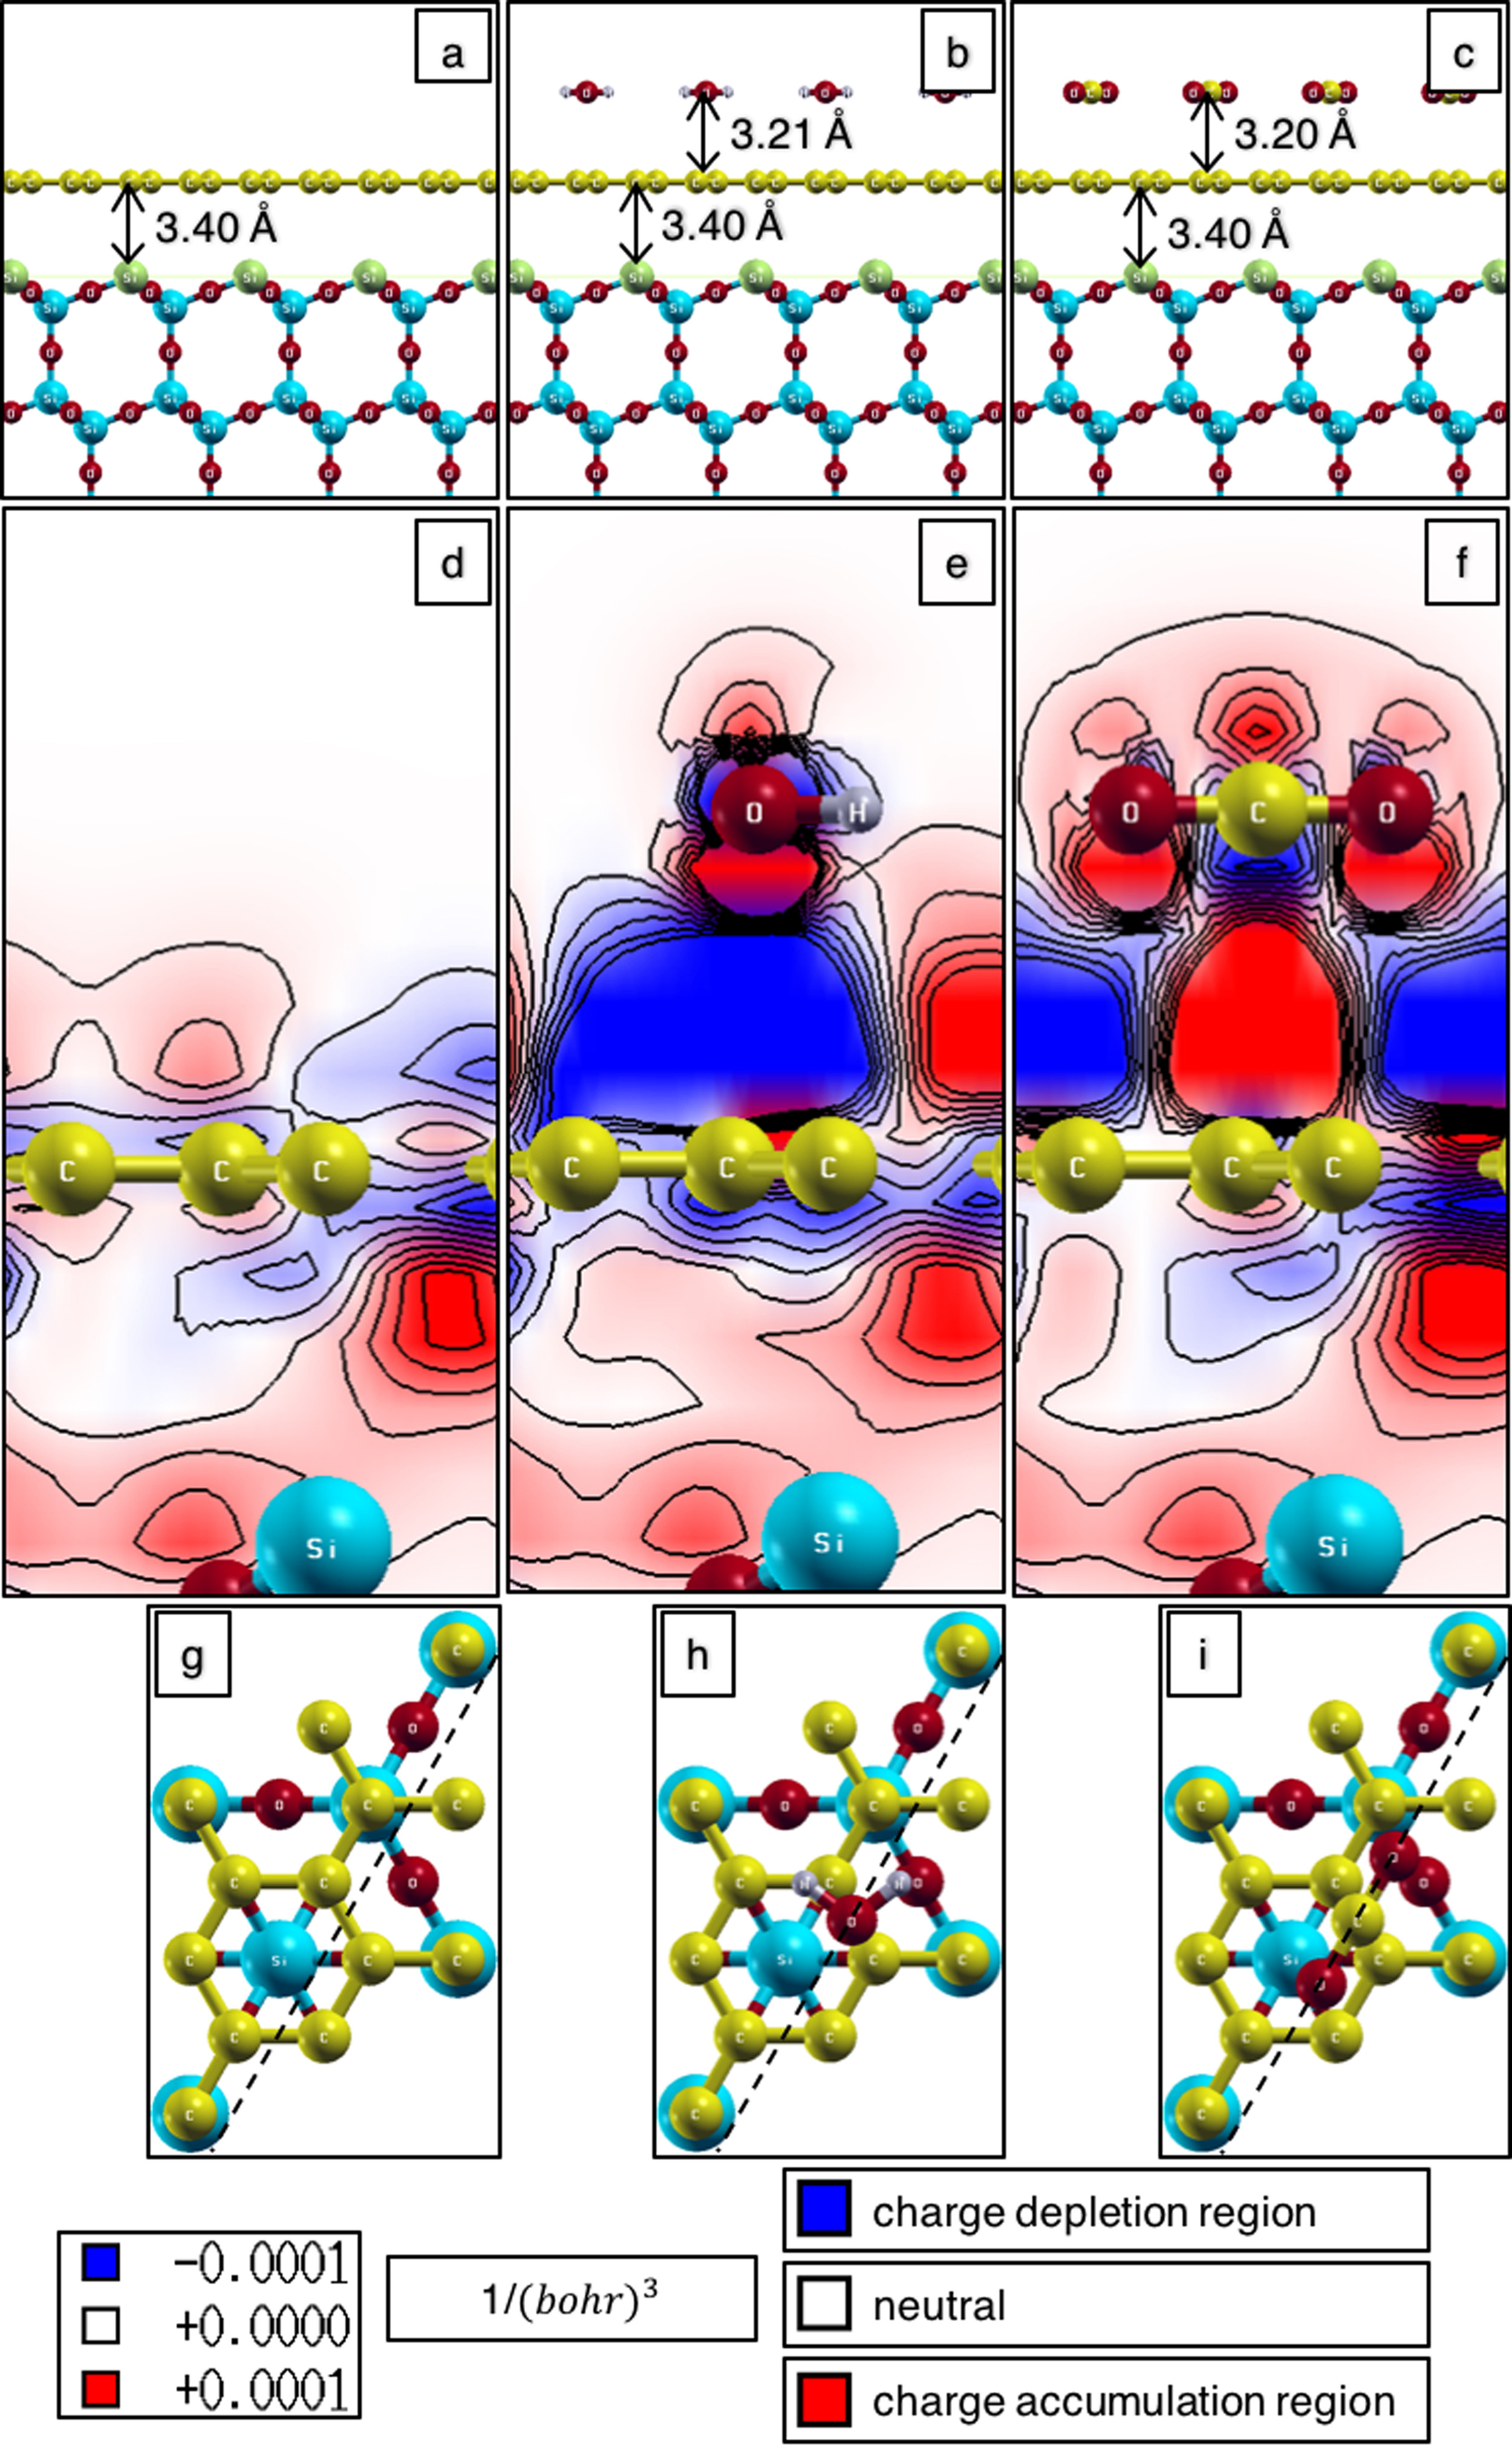
\includegraphics[scale=0.9,keepaspectratio]{Figs/Paper1a.jpg} %[width=\textwidth]
    \caption{excerpt from manuscript describing Paper \hyperref[P1]{$\Rmnum{1}$}~\cite{Elgammal2017}.}
    \label{paper1a}
\end{figure}

Our findings were in line with literature~\cite{Wehling2008}, where the weak interaction between the adsorbate molecules on top of the pristine graphene sheet and the defect states arising from the underlying substrates induces a doping effect in the graphene sheet. That is detailed in Paper \hyperref[P1]{$\Rmnum{1}$}, where the substrate defects effect when combined with water molecules, change the electronic structure properties represented by CDD contours. We studied the substrate defects on three different substrates and found that doping effect took place in all the substrate surface defect types across the three different substrates with different degrees. The substrate slabs were either of silica type ($\beta$-cristobalite and $\alpha$-quartz) or $\alpha$-sapphire. Notably, the defects within the $\beta$-cristobalite substrate surface were the $Q_{\textrm 3}^{\textrm 0}$,  which is a well-known and common silica substrate surface defect~\cite{Wilson2000, Walsh2000}. The defects within the other silica and sapphire substrates type took place at the substrates' surface with either silicon or aluminium undercoordinated atoms terminating the substrates. We referred them to as Si-terminated $\alpha$-quartz (0001) and Al-terminated sapphire (0001) substrates. The respective (CDD) contour plots are available in Fig. \ref{paper1a}, Fig. \ref{paper1b} and Fig. \ref{paper1c} for the three cases respectively.

\begin{figure}
    \centering
    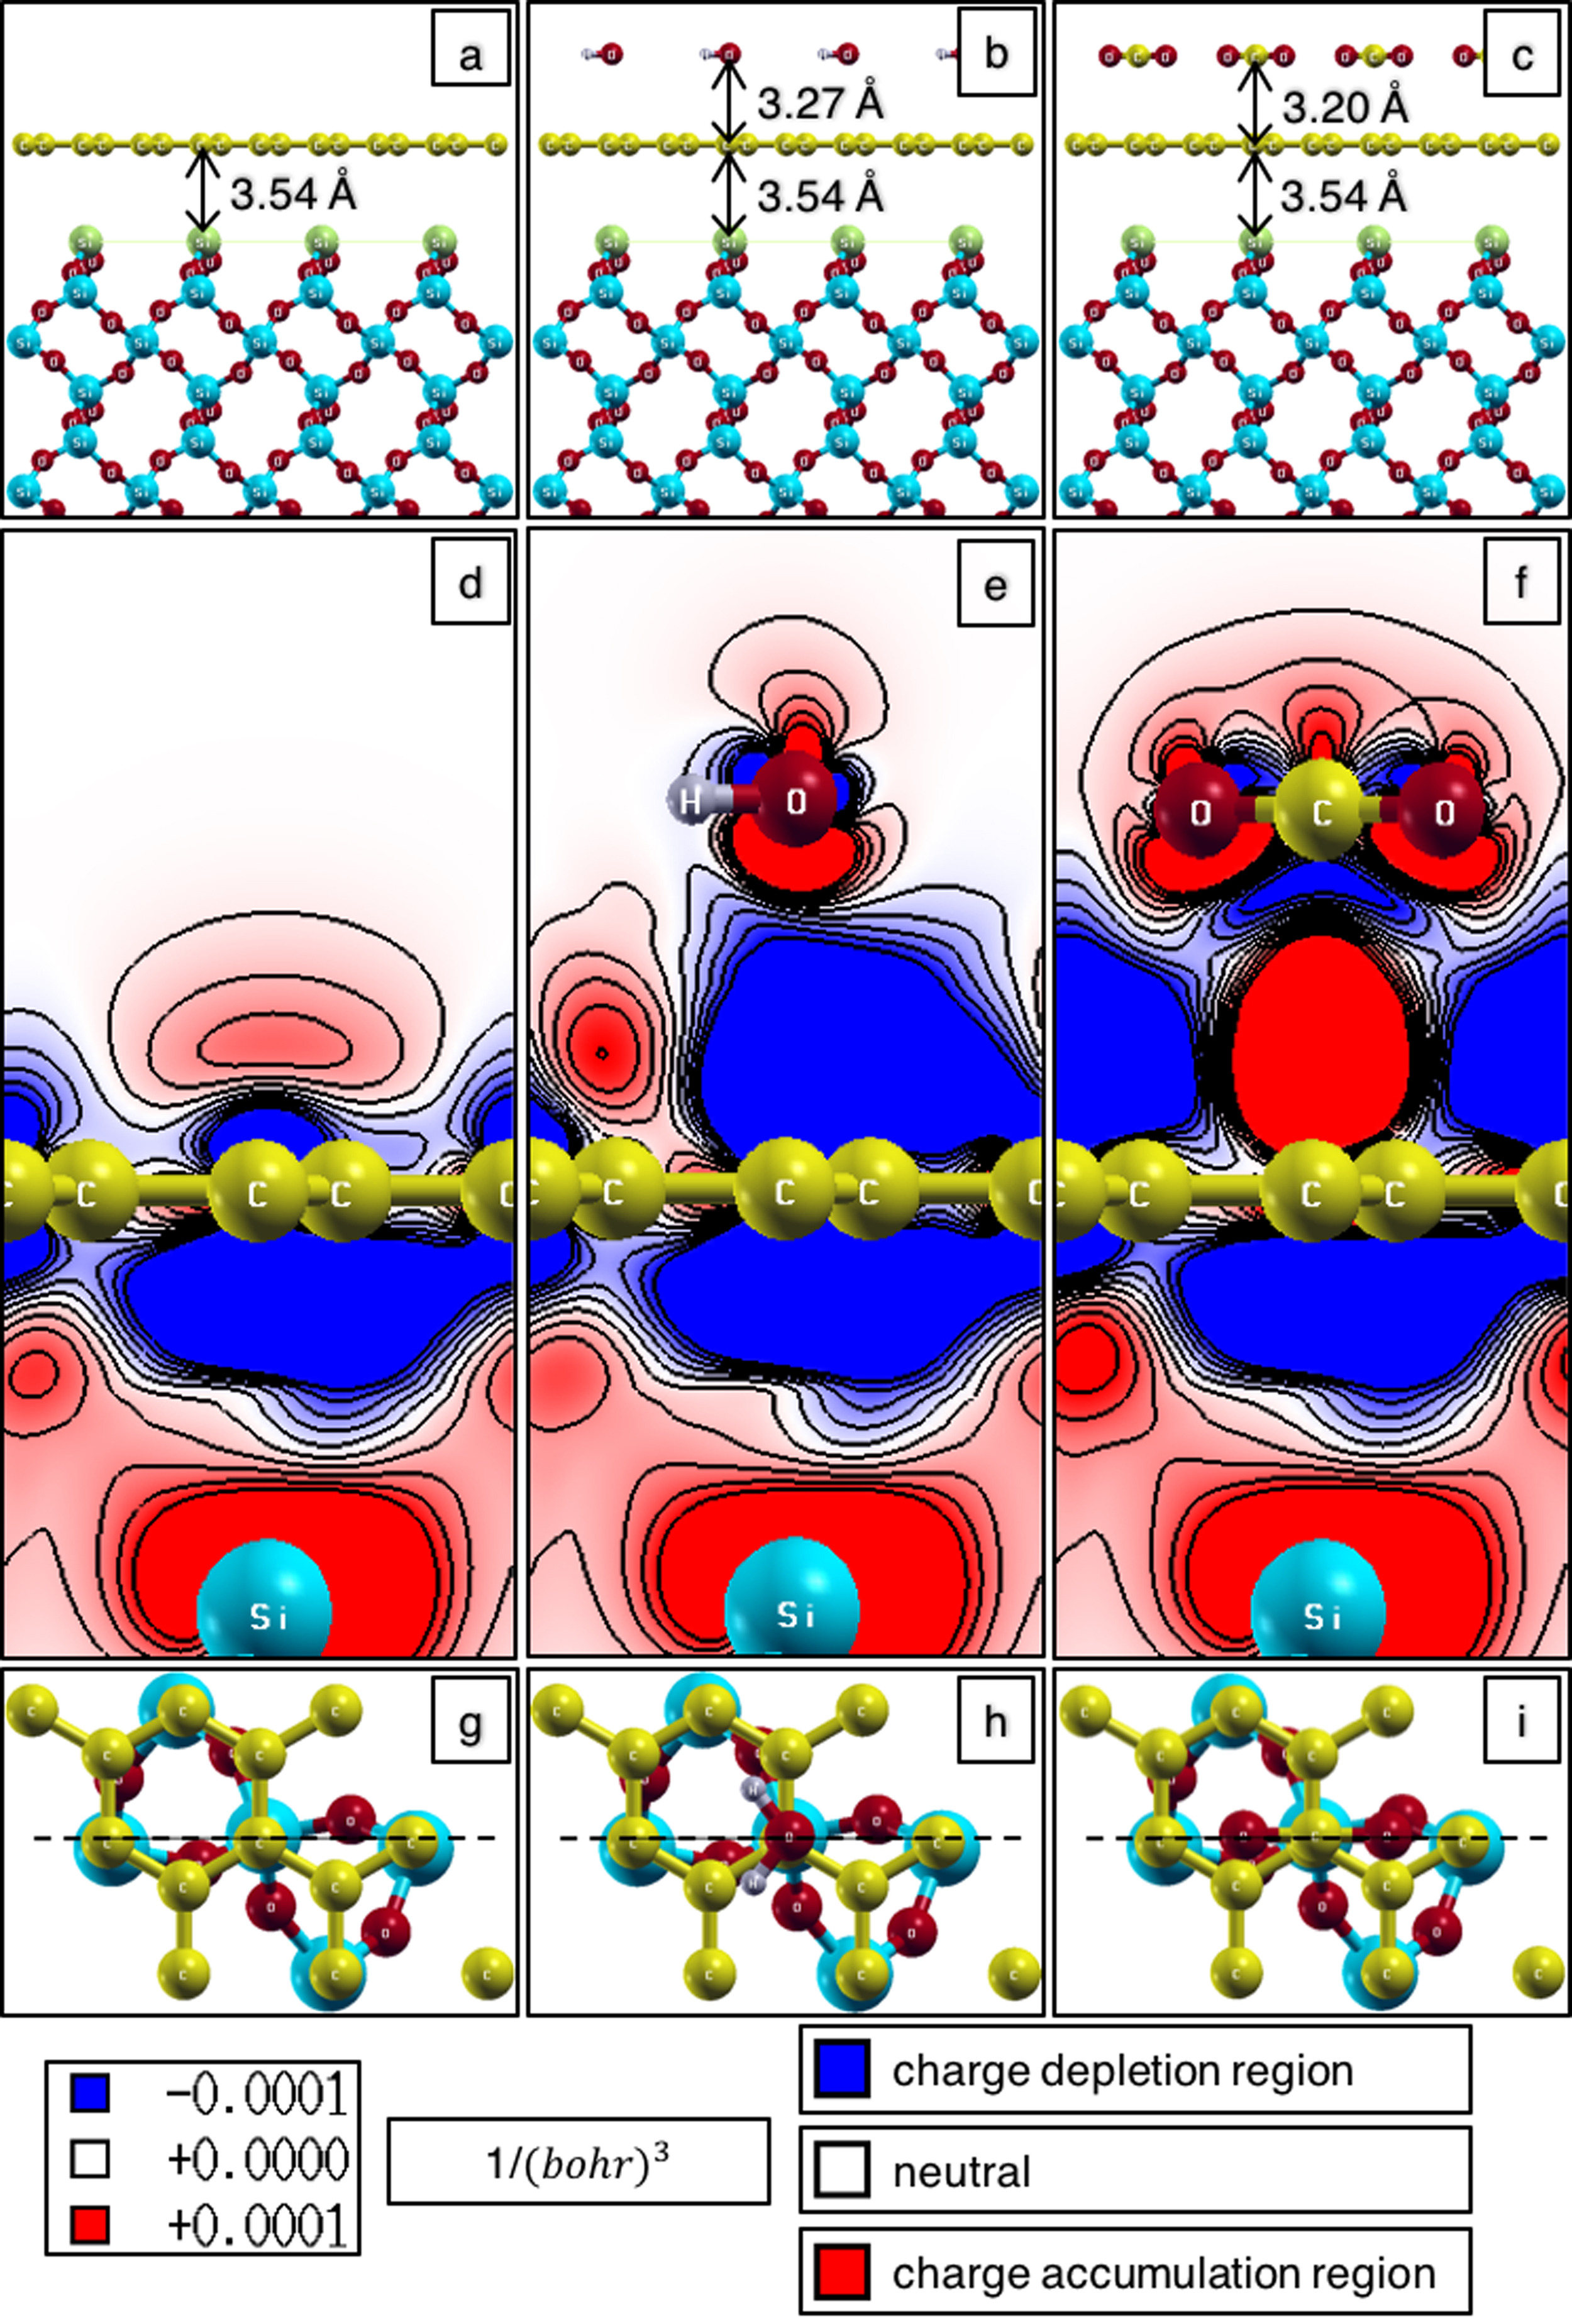
\includegraphics[scale=0.9,keepaspectratio]{Figs/Paper1b.jpg} %[width=\textwidth]
    \caption{excerpt from manuscript describing Paper \hyperref[P1]{$\Rmnum{1}$}~\cite{Elgammal2017}.}
    \label{paper1b}
\end{figure}

\begin{figure}
    \centering
    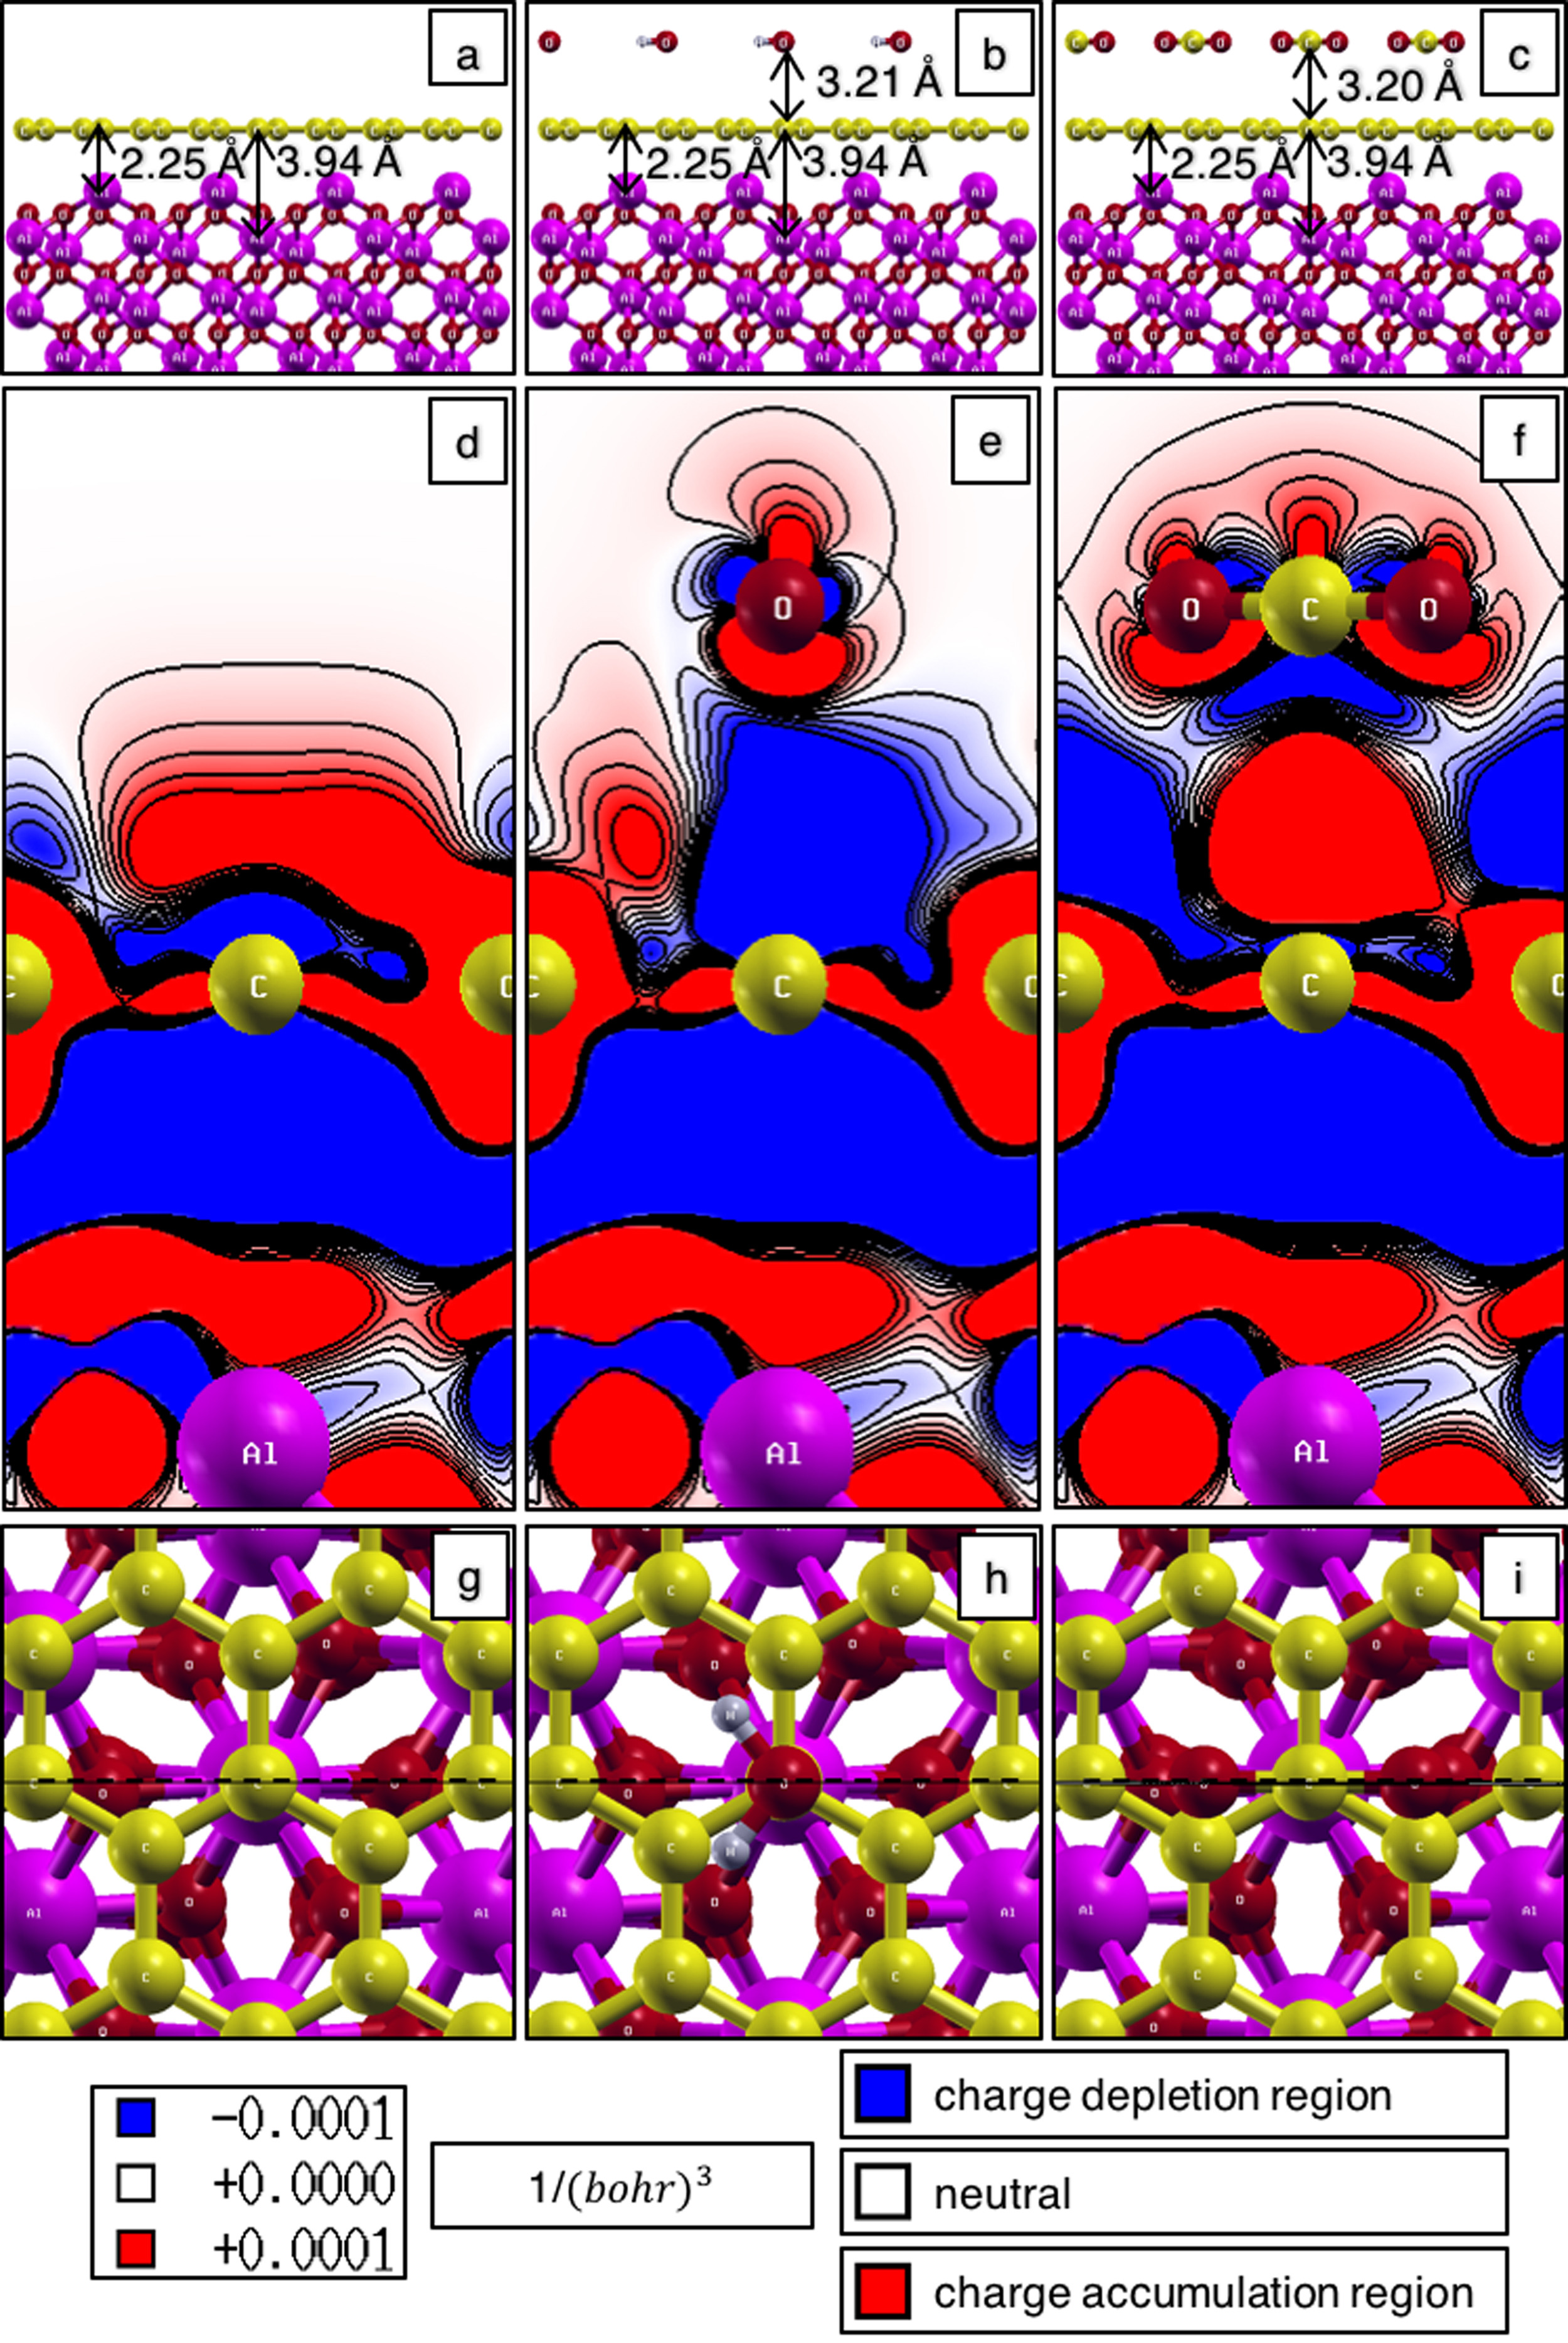
\includegraphics[scale=0.9,keepaspectratio]{Figs/Paper1c.jpg} %[width=\textwidth]
    \caption{excerpt from manuscript describing Paper \hyperref[P1]{$\Rmnum{1}$}~\cite{Elgammal2017}.}
    \label{paper1c}
\end{figure}

In paper \hyperref[P1]{$\Rmnum{1}$}, we examined several adsorbate configurations, distinguished by the relative (x-y) plane positioning of the adsorbates with respect to the graphene sheet. Among all the relaxed configurations, adsorbate configurations with the lowest energy (a preferred configuration) are the closest to the graphene sheet among the same substrate type. This observation is due to a stronger bonding (more hybridisation) that result in a shorter bonding distance. We found that water adsorbates always preferred to be above the centre of the graphene hexagon (hollow sites) regardless of the type of the underlying substrate. Meanwhile, carbon dioxide adsorbates preferred configurations differed according to the substrate. For the cristobalite case: it was on top of the midway between two carbon atoms (the so-called bridge position). For the quartz case: it was on top of silicon atom of the Si-terminated substrate. For the sapphire case: it was on top of a carbon atom in the graphene sheet as well as an aluminium atom (inside the substrate and not the substrate's surface top atom). Moreover, carbon dioxide adsorbates revealed a binding distance of 3.2 Å away from the graphene sheet in all the preferred configurations across all the three cases. We extended this study with paper \hyperref[P2]{$\Rmnum{2}$} taking into consideration a more robust treatment of the dispersion interactions using non-local vdW functionals that we previously discussed in Chapter \ref{DFT-chapter}. As a follow-up, we studied graphene's electronic structure properties being in contact with a different pool of substrate types which can be metal, semiconductor or insulators as in manuscript \hyperref[P3]{$\Rmnum{3}$}. Moreover, we found good agreement with experimental equilibrium distances and binding energies (or adhesive energies).
\clearpage
In summary, upon studying those different systems, we can conclude that, with the presence of the adsorbates, the doping effect differs slightly per different types of adsorbates within the silica substrates, while it differs dramatically in comparison with sapphire substrate type. Sapphire can be embedded as a coating material silicon substrates~\cite{Jadaun2011}. Thus, we can conclude that the effect of adsorbates existence on the graphene sheet can depend heavily on the substrate properties, types and its associated defects as previously reported in~\cite{Wehling2008}.

\begin{figure}
    \centering
    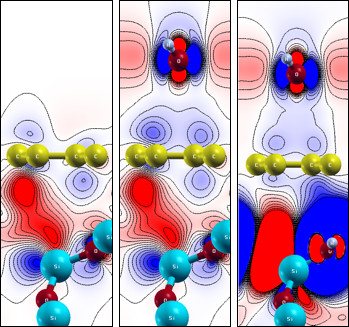
\includegraphics[width=\textwidth]{Figs/Paper4.png}
    \caption{excerpt reprinted from manuscript describing Paper \hyperref[P4]{$\Rmnum{4}$}~\cite{Smith2015}.}
    \label{paper4}
\end{figure}

In Papers \hyperref[P4]{$\Rmnum{4}$}, \hyperref[P5]{$\Rmnum{5}$}, we studied similar systems to the ones in Papers \hyperref[P1]{$\Rmnum{1}$}, \hyperref[P2]{$\Rmnum{2}$} in conjunction with experimental input. We showed in both articles a qualitative overview on the influence of substrate-surface defects on pristine graphene sheet with either water or carbon dioxide molecules adsorbed on top. The results showed a difference in the charge distribution when comparing cases lacking adsorbates with cases of adsorbates existence as shown per Figs. (\ref{paper4}), (\ref{paper5}). Besides, there is a difference in the CDD contours according to the surface conditioning, as we examined cases of hydrogen-passivated and non-passivated surface termination as shown in Fig. (\ref{paper4}). The CDD contours experience alternating charge depletion and accumulation regions throughout the graphene sheet depending on the different ambient condition it can coexist according to the examined cases.

\begin{figure}
    \centering
    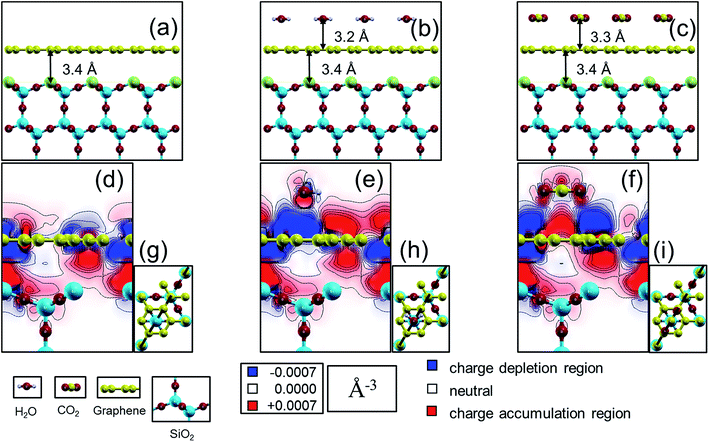
\includegraphics[width=\textwidth]{Figs/Paper5.png} %[scale=0.5,keepaspectratio]
    \caption{excerpt from manuscript describing Paper \hyperref[P5]{$\Rmnum{5}$}~\cite{Smith2017}.}
    \label{paper5}
\end{figure}

We expanded the study to double layered graphene, which has caught interesting properties leading to useful utilisation in sensor devices~\cite{Melios2016, Yakovkin2016}. We performed a related joint-experimental study in~\cite{Xuge2017} via DFT calculations on pristine double layered graphene residing on one type of $\alpha$-quartz substrate. The CDD contour plots depicted in Fig. (\ref{paper6}) revealed that the double-layered graphene isolates the combined doping effect of the substrate and the adsorbates, that we already discussed before. Each layer is concerned with the adhered weakly-bounded system which are the substrate and the adsorbates. Furthermore, the overall charge transfer was also small, signalling value of 0.05e and 0.04e as a net charge transfer towards the adsorbate molecules of carbon dioxide and water molecules.

\begin{figure}
    \centering
    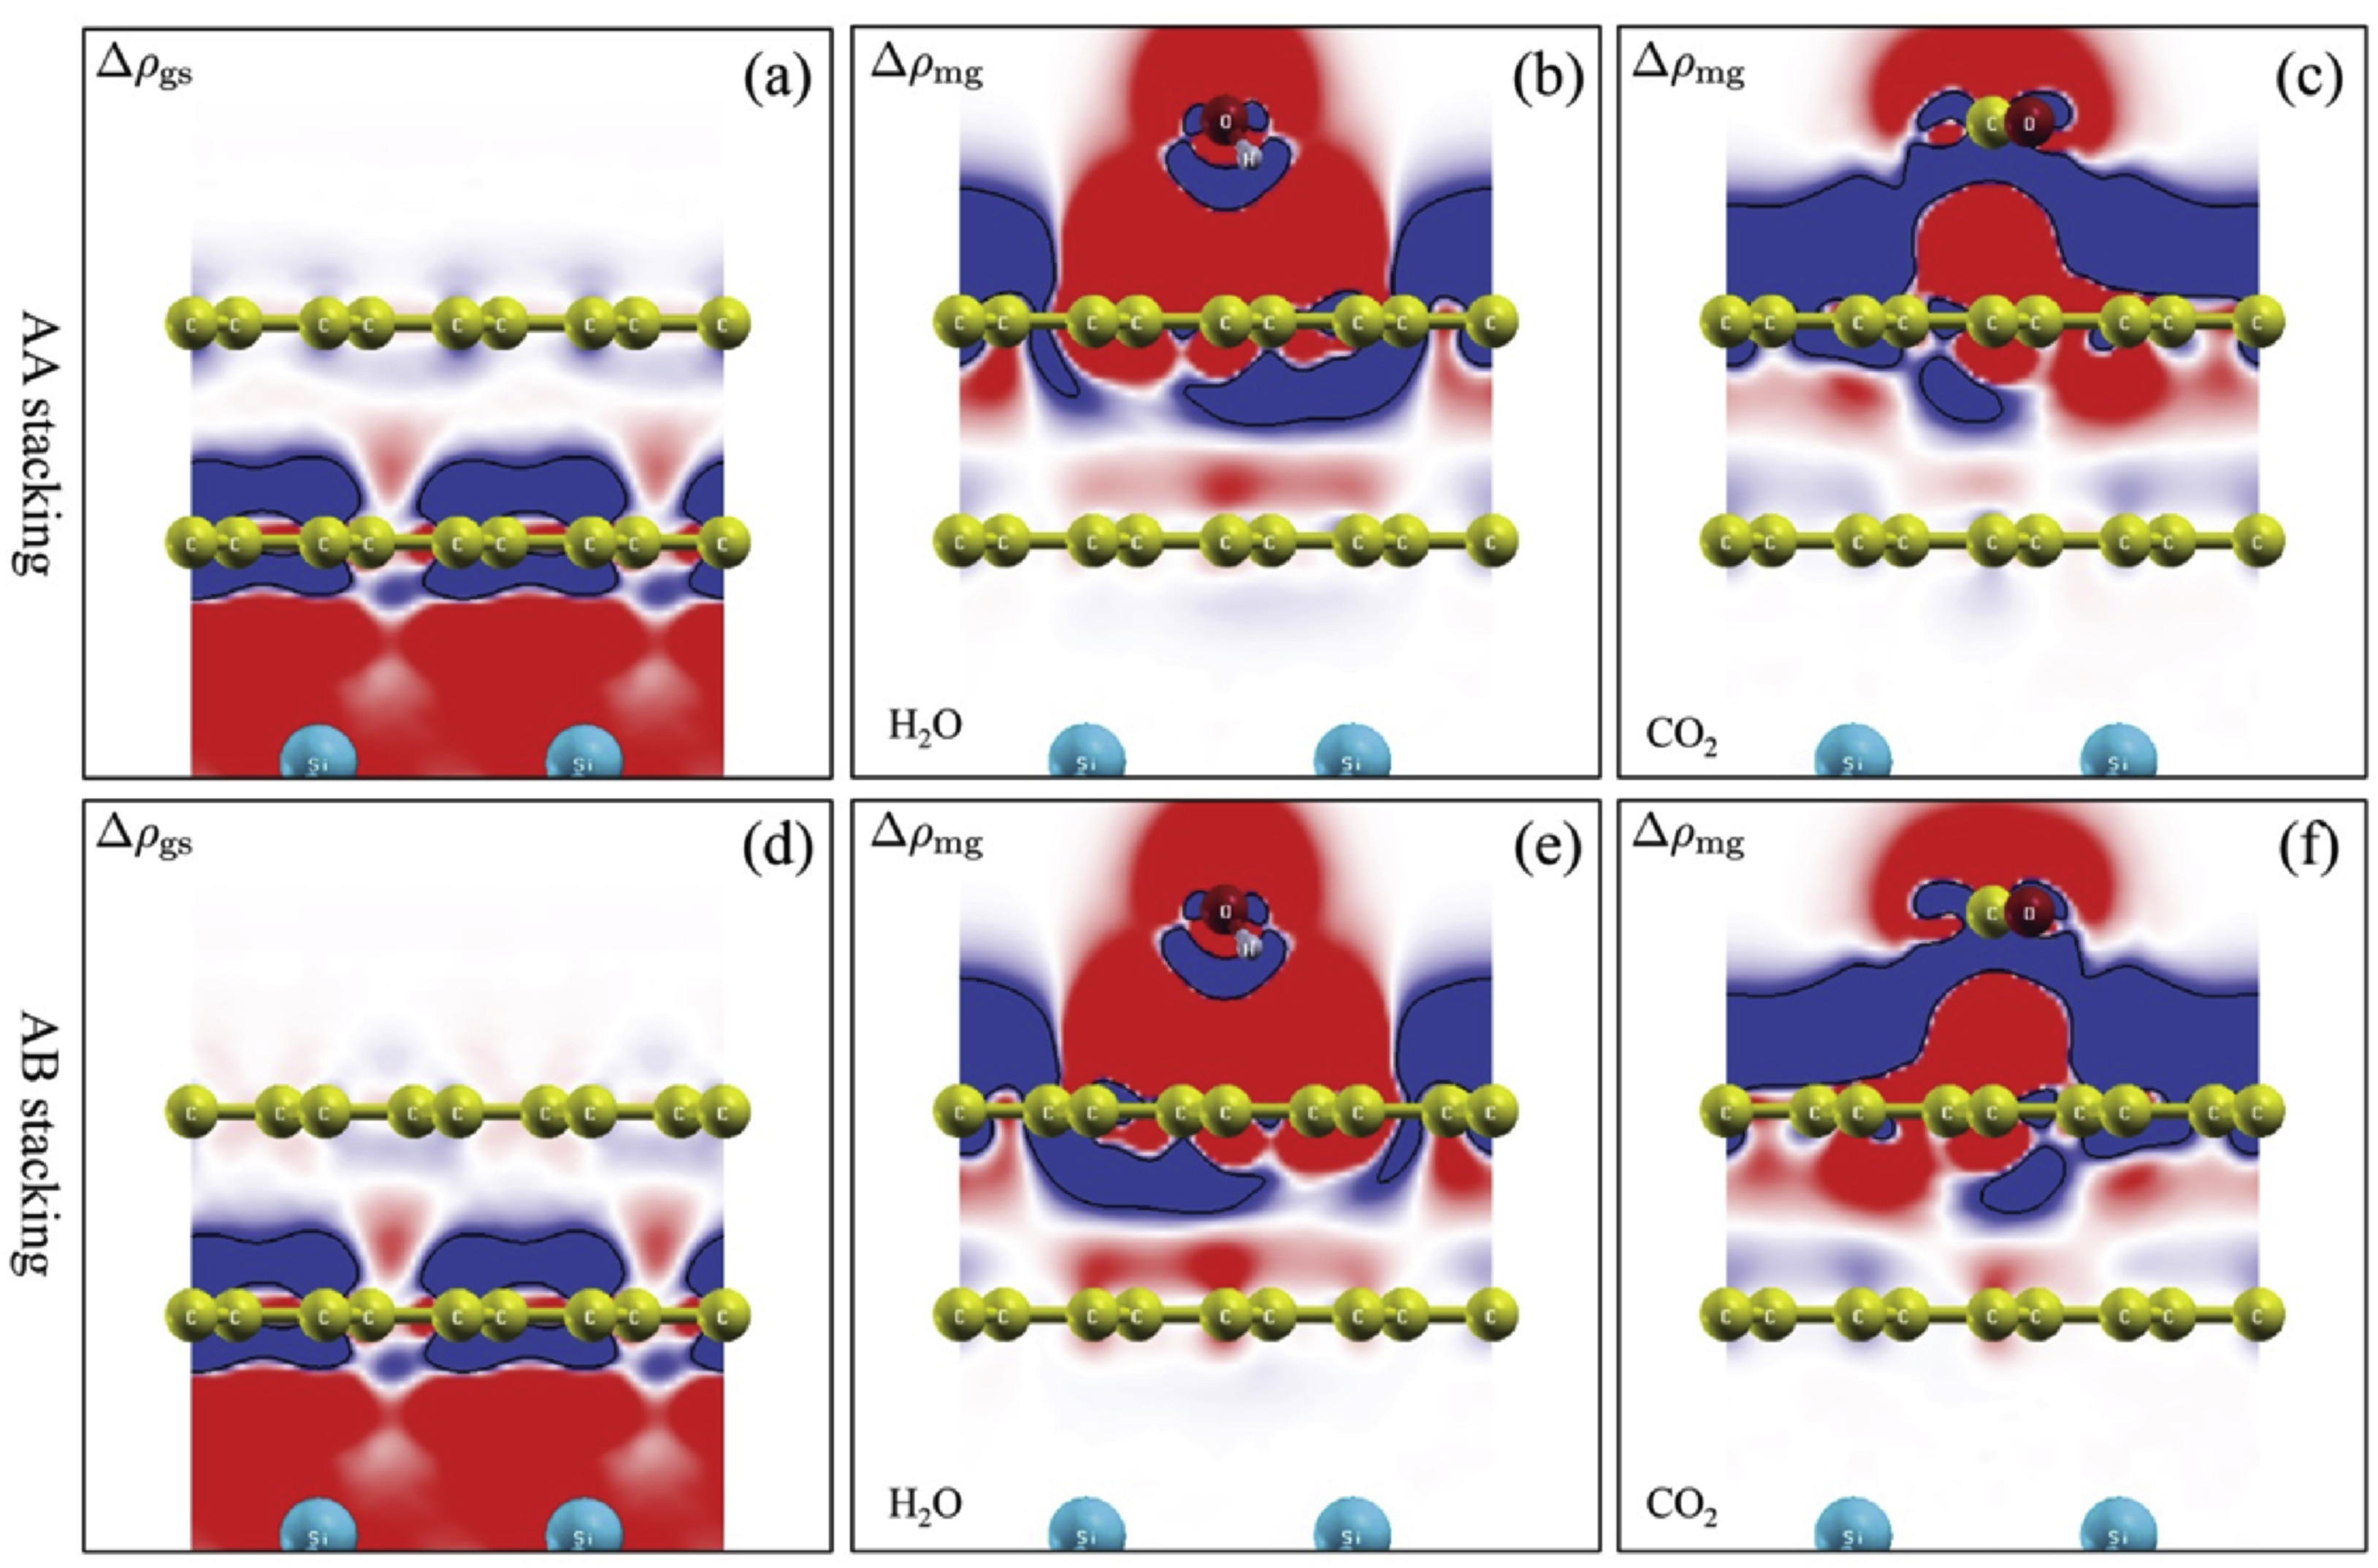
\includegraphics[width=\textwidth]{Figs/Paper6.jpg} %[scale=0.8,keepaspectratio]    
    \caption{excerpt from manuscript describing Paper \hyperref[P6]{$\Rmnum{6}$}~\cite{Xuge2017}.}
    \label{paper6}
\end{figure}

As the ultimate goal of designing such devices is to obtain higher value systems according to the \textit{more than Moore} paradigm we pointed to in Chapter \ref{introduction}, we need to isolate different components and functionalities on the same chip in order not to interfere with each-other and comply with the targeted diversification purpose. Thus, we performed a combined experimental and theoretical study as in~\cite{Smith2016} for confirming the passivating layers effect on the graphene-based sensors and how the associated CDDs looks like as rendered in Fig. \ref{paper7}. We showed with an availability of a passivation layer in between the graphene and adsorbates that the adsorbates effect on the graphene sheet is dysfunctioned.

\begin{figure}
    \centering
    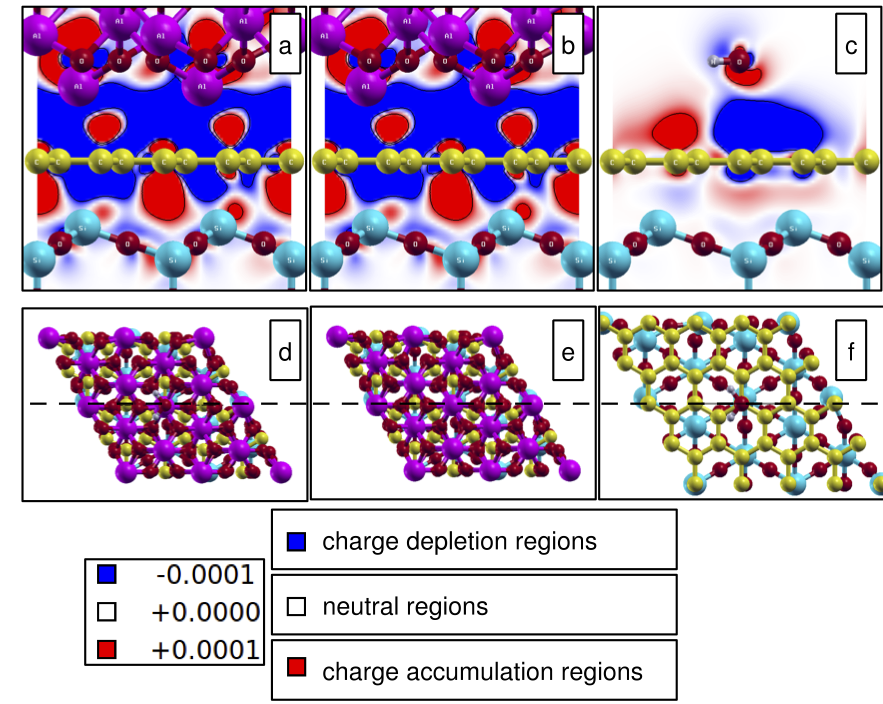
\includegraphics[width=\textwidth]{Figs/Paper7.png}
    \caption{excerpt from manuscript describing Paper \hyperref[P7]{$\Rmnum{7}$}~\cite{Smith2016}\textcopyright 2016 IEEE.}
    \label{paper7}
\end{figure}
\endinput
\chapter{Conclusions and future outlook} 
In this work, we discussed a theoretical investigation of a possibly \textit{more than Moore} application of graphene's sensitivity towards humidity and carbon dioxide molecules. 

We focused on extracting the electronic structure properties of single-layered pristine graphene as a sensor, more especially as humidity and carbon dioxide sensors. Similarly, we extended the studies towards investigating the double layered graphene sensing action towards the same adsorbates. We demonstrated the effect of passivation on such sensing action resulting in dysfunctioning sensors for better integrity of high valued systems in the \textit{more than Moore} paradigm. All in all, we consider this approach crucial for optimal delivery of high-valued systems combining system-on-chip (SoC) with system-in-package (SiP) as direct usability and applicability of \textit{more than Moore}.

In particular, we performed the studies on graphene within different ambient conditions through first-principle \textit{ab-initio} calculations. We focused on the combined effect of the underlying substrates and adsorbates on top of the graphene sheet itself. This effect is attributed to be a doping effect which is responsible for different adhesive forces added to the graphene's interface with the substrate as well as to the adsorbates on top. These results are in line with related literature available in~\cite{Wehling2008, Liu2008, Levesque2011, Anton2012, Hong2016, Ashraf2016, Melios2017}. Those interactions are weak and governed mainly by van der Waals forces. Thus, the study also included different investigations of such weak interaction of graphene on different surfaces with metal, semiconductor and insulator nature where physisorption or chemisorption adhesive nature govern graphene's adhesion with those substrates. 

In summary, we demonstrated and highlighted some factors that affect the sensing behaviour of pristine graphene where the electronic structure of such graphene-adsorbates interactions relies on the stacking orders as well as the underlying substrate-induced doping effect due to common defects available on the substrate surfaces. 

As future work, expanding the study to involve other molecules' combined effect with the substrates via accurate van der Waals methods is an important step towards incorporated into more sensing devices. Examining other 2D materials can have potential interest opening more applications for gas sensory paradigm~\cite{Yue2013, Zhao2014}, especially if they feature either direct or indirect bandgaps. Moreover, studying the conductance employing transport calculations within the non-equilibrium Green's functions scheme~\cite{DattaAtomstotransistors} is crucial for ultimate benchmarking purposes and to explore the transport properties of such sensing devices from a purely theoretical point of view. Finally, merging results from multi-scale simulation paradigm and \textit{ab-initio} can be useful for understanding more properties of such systems in-design~\cite{fiori}.
\endinput



%%%
 \bibliographystyle{apsrev4-1} %unsrt %apsrev4-1
 %\newpage
 
 \bibliography{thesisRefs}{}
%%%

\end{document}
\endinput
